%% 美赛模板:正文部分

\documentclass[12pt]{article}  % 官方要求字号不小于 12 号,此处选择 12 号字体
% 本模板不需要填写年份,以当前电脑时间自动生成
% 请在以下的方括号中填写队伍控制号
\usepackage[2513946]{easymcm}  % 载入 EasyMCM 模板文件
\usepackage{ctex}
\usepackage[pages=some]{background}
\backgroundsetup{           % I insert it in the "title_page.tex" file
 scale=1,
 angle=0,
 opacity=.1,  %% adjust
 contents={
\includegraphics[width=\paperwidth,height=\paperheight]{bg.png}}
 }
\usepackage{ulem} % 提供下划线功能
\usepackage{placeins}

\problem{E}  % 请在此处填写题号
%\usepackage{mathptmx}  % 这是 Times 字体,中规中矩 
\usepackage{mathpazo}  % 这是 COMAP 官方杂志采用的更好看的 Palatino 字体,可替代以上的 mathptmx 宏包
\title{From Forest to Farmland: the Cascading Effects of Ecological Transition and Organic Agriculture}  % 标题

% 如需要修改题头(默认为 MCM/ICM),请使用以下命令(此处修改为 MCM)
%\renewcommand{\contest}{MCM}

% 文档开始
\begin{document}

% 此处填写摘要内容
\begin{abstract}
    In our work, We divided the topic into four tasks and logically modeled 
    the farmland ecosystem based 
    on various conditions. \textbf{At the final stage, we innovatively employed 
    the Monte Carlo method to test the stability of the model, and meticulously 
    discovered its significant analytical value}. Below is a more detailed 
    introduction:

For task 1,We use \textbf{Lotka-Volterra Model} to develop the \textbf{FarmModel-V1} model. 
We consider the basic food web and the use of \textbf{herbicide} and \textbf{pesticide}. 
Based on this, we introduce pesticide \textbf{pulse functions}, pesticide 
\textbf{volatilization functions}, as well as \textbf{resistance} and \textbf{seasonal growth 
rate variation factors}, to build the FarmModel-V1 model. The model 
indicates the weeds will dominate the system,leading to the extinction
 of other species.

For task 2, We take beneficial soil organisms BC and species A into 
consideration and develop the \textbf{FarmModel-V2} model. We analyze the impact 
of \textbf{species restoration} on the ecosystem and find that BC could not change
 the situation in task1. However, introducing species A effectively 
 balances the weed population leading to the stability of whole ecosystem.

For task 3,We remove pesticides in FarmModel-V2 and find the crops decrease 
significantly. Then, we introduce  species such as bats and bees to
 keep the ecosystem balance, developing the \textbf{FarmModel-V3} model. The 
 results show that both \textbf{bats} and \textbf{bees} effectively balance the weed 
 population, increase the population of crops and other species, and 
 enhance the farm's yield from 500 to 3500(Bat) and 1700(Bee).

For task 4,we establish the \textbf{Green Agriculture Index} to measure the 
impact of organic farming. The index is constructed by four 
aspects:soil,aquatic environment, air and biodiversity.The 
weights are calculated using \textbf{EWM}, and they are \textbf{22\%,17\%,19\%,42\%}.
Then we use \textbf{Monte Carlo simulation} to compare the profit of green 
agriculture with conventional one, finding green agriculture has
 better economic benefits.

Additionally, to simulate real natural conditions, we developed the 
\textbf{FarmModel-V3$_{\alpha,\beta,\gamma}$} models, by introducing natural 
disasters such as drought, floods, and pest outbreaks to assess the 
stability of the ecosystem under natural shocks. The results indicate 
that the ecosystem could recover relatively quickly after natural 
disasters,improving its stability. And we conduct a \textbf{Monte Carlo 
simulation} for the growth rate of weed$(r_W0)$ and crop$(r_C0)$ to 
obtain the species distribution one year later. For model 1, we found 
a \textbf{“boundary line” ($\bold{r_W0 = 0.407r_C0 + 0.125}$)}.In the scenarios on 
either side of this line, the ecosystem is dominated by either weeds 
or crops.For model 3, we use the results to construct indicator of 
"output performance" and "risk".We use the indicators to describe model3's three stages as \textbf{(0.26, 0.27)}, \textbf{(0.79, 0.19)}, and \textbf{(0.54, 0.22)}. 
Ultimately, we conclude that the system without pesticides and with 
the introduction of bats have the best output performance and lowest 
risk.

    \vspace{5pt}
    \textbf{Keywords}:Lotka-Volterra Model\quad Organic Agriculture\quad Monte Carlo Simulation

\end{abstract}

\maketitle  % 生成 Summary Sheet
\tableofcontents  % 生成目录


% 正文开始
\section{Introduction}
\subsection{Background}
The conversion of forests into agricultural ecosystems exerts a 
profound impact on biodiversity, soil health, and ecosystem 
services. During agricultural expansion, the complex food webs 
in forests, which are crucial for maintaining ecological balance, are frequently replaced by monoculture farming and intensive chemical applications. This transformation disrupts natural systems, resulting in a series of ecological consequences.

The initial forest clearing fragments habitats, causing a decline in native species such as birds and insects. Chemical usage further upsets the ecological equilibrium. However, over time, edge habitats may recover, allowing species to reestablish and ecological stability to be achieved. For instance, bats, being insectivores and pollinators, play a vital role in pest control and biodiversity support.

To better analysis the transformation of forests into farmlands, 
many researchers have developed models to simulate the dynamics 
of agricultural ecosystems. For example, 
the Lotka - Volterra model, fundamental for predator - prey dynamics
, has been widely applied. Previous studies, like Demir (2024) 
using delay differential equations to account for time-delay 
effects \cite{Demir2024}, Blake (2024) analyzing the influence of 
agricultural interventions such as pesticides \cite{Blake2024}, 
Adenekan (2024) exploring extensions considering spatial and 
temporal dynamics due to complex agricultural practices 
\cite{Adenekan2024}, and Dandekar et al. (2024) proposing 
an improved model by integrating scientific machine learning 
methods \cite{Dandekar2024}, have made remarkable achievements. 
However, they often focus on individual aspects and lack a 
comprehensive view of overall ecosystem changes.


\subsection{Problem Restatement}
In this problem, as members of the Consideration of Mature Agricultural 
Practices (COMAP) group, we are required to construct a model to track the 
habitat changes during the process of forests being converted into farmlands. 
We need to explore how the transformed forest areas change over time with 
the evolution of the ecosystem and the formulation of agricultural decisions. 
The analysis must take into account both natural processes and human decisions.

During the modeling process, we need to simulate the current new agricultural 
ecosystem. Construct a basic food web model, identify the producers and 
consumers therein, and consider the impact of the agricultural cycle and 
its seasonality on the dynamic changes of the ecosystem. Meanwhile, we should 
study the impact of the reemergence of species on the ecosystem by 
incorporating two different species into the model for analysis. 
Additionally, we need to evaluate the impact of herbicides and pesticides 
on the ecosystem. Finally, we need to analyze the impact of organic 
agriculture on the ecosystem.

To sum up, we divide the problem into four tasks:
\begin{itemize}
\item Task 1: Construct a basic food web model and analyze the evolution of the farmland ecosystem under normal circumstances.
\item Task 2: Consider the species reemergence process and explore the impact of species restoration on the farmland ecosystem.
\item Task 3: Explore the benefits of adopting organic agriculture (introducing organisms) to the ecosystem under the condition of pesticide absence.
\item Task 4: \textbf{Go Green} Based on the previously established model, analyze how to employ strategies of green agriculture to optimize both ecological and economic benefits.
\end{itemize}

\subsection{Our Work}
To solve the problem and deeply study how agricultural ecosystems change 
and behave over time.
we started with existing research but added new ideas and improvements. 
We looked at both natural processes and human decisions. Here is what we did:

\begin{enumerate}[\bfseries 1.]
    \item To address \textbf{Task 1}, we developed the \ref{eq:FarmModel-V1}.
    
    We began by considering the simplest scenario, where only 
    crops, weeds, and pests interact, and the concentrations of 
    herbicides and pesticides remain constant. Under these assumptions, 
    we initialized the model. That is \textbf{FarmModel-V0}.
    Building on this, we introduced additional complexities to better 
    reflect real-world agricultural practices, including a pesticide 
    pulse function, a pesticide volatilization function and the incorporation of 
    pesticide resistance and seasonal growth rate variations.By doing so, we 
    developed \ref{eq:FarmModel-V1}.
    

    \item To address \textbf{Task 2}, we introduced species A and B as 
    representatives of species reemergence. By modeling their interactions, 
    we developed \textbf{eq:FarmModel-V2} and conducted analysis and discussion.

    \item To address \textbf{Task 3}, we developed the \textbf{FarmModel-V3}. 
    
    We attempted to remove the effects of 
    pesticides in \ref{eq:FarmModel-V2} to 
    observe how the ecosystem would change under this condition. 
    And then, we introduced the concept of organic farming by 
    incorporating organisms such as bats and bees to regulate the balance of 
    the ecosystem. By modeling the interactions of these introduced species, 
    we simulated the dynamics among various variables, resulting in \textbf{FarmModel-V3}
    

    \item To address \textbf{Task 4}, we establish the Green Agriculture Index to measure the 
    impact of organic farming. The index is constructed by four aspects:soil,aquatic environment, air and biodi-
    versity.Then we
    use Monte Carlo simulation to compare the profit of green agriculture with conventional
    one.

    \item At last, we have innovatively proposed methods for disaster reliability testing and Monte Carlo stability testing.
    At the same time, this further aids us in gaining a deeper understanding of the problem.

    
\end{enumerate}

The following table is our overall framework:

\begin{figure}[h]
    \centering
    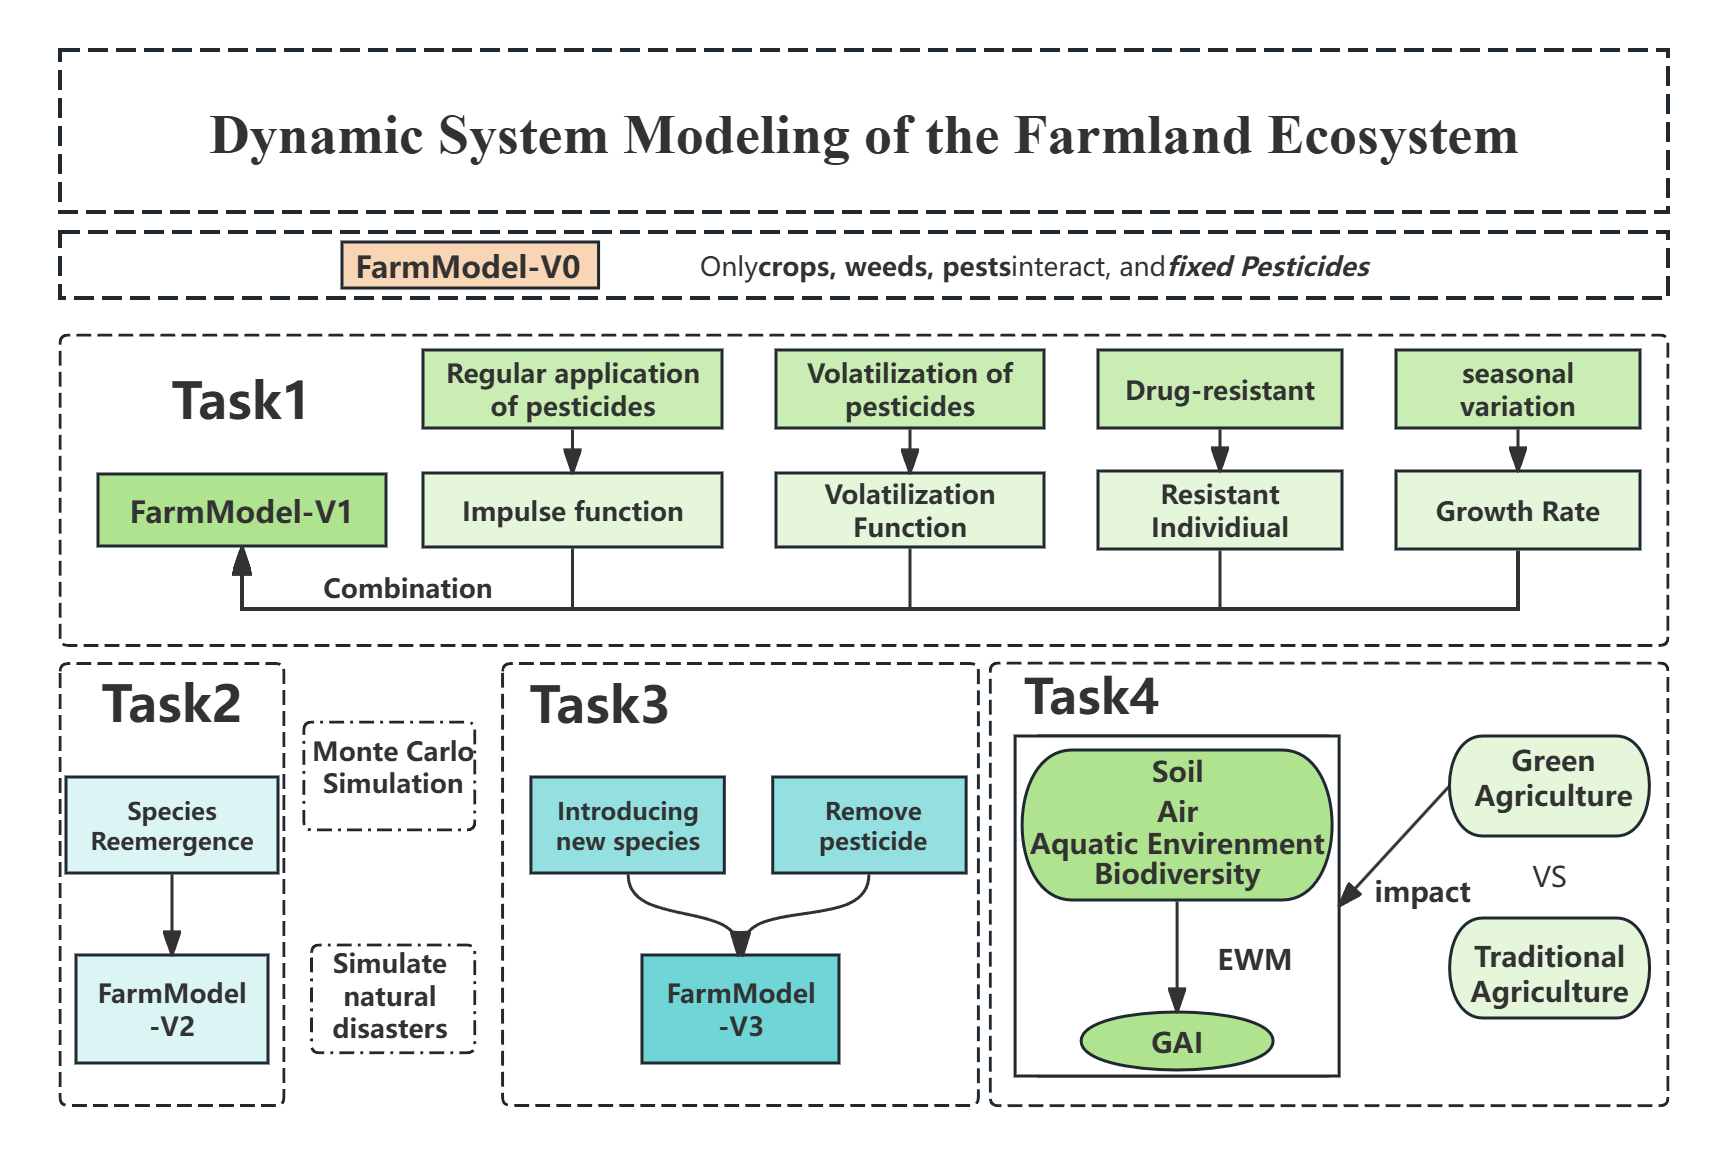
\includegraphics[width=0.9\textwidth]{2025美赛E.png}
    %\caption{The overall framework of our work.}
    \label{fig:framework}
\end{figure}




\section{Assumptions and Notations}
\subsection{Assumptions}
To simplify the problem, we make the following assumptions:
\begin{itemize}
    \item\textbf{Assumptions 1:} We use crops, weeds, bats, and 
    herbivorous insects as representatives of the organisms in the 
    agricultural ecosystem. Unless otherwise specified, we do not 
    consider the impact of other organisms.
    \item\textbf{Assumptions 2:} We assume that there is no migration 
    of organisms into or out of the ecosystem during the study period.
    \item\textbf{Assumptions 3:} Unless otherwise specified, we do not 
    consider the impact of drastic environmental changes on the population 
    of organisms.
    \item\textbf{Assumptions 4:} We ignore the role of microorganisms, 
    soil, and other non-animal and non-plant organisms in the ecosystem.
    \item\textbf{Assumptions 5:} We assume that pest only prey on crops.
    \item\textbf{Assumptions 6:} We assume that all indicators are 
    continuous with respect to time.
\end{itemize}
\subsection{Notations}
The primary notations used in this paper are listed in Table \ref{tb:notation}.

% 三线表示例
\begin{table}[htbp]
    \begin{center}
    \caption{Notations}
    \renewcommand{\arraystretch}{1.5} % 将行间距增大为原来的 1.5 倍
    \begin{tabular}{cc}
        \toprule
        \multicolumn{1}{m{3cm}}{\centering Symbol}
        &\multicolumn{1}{m{8cm}}{\qquad\quad Definition}\\
        \midrule
        $t$ &  time elapsed since the conversion of forest to farmland \\
        $C$ & quantity of crops \\
        $W$ & quantity of weeds \\
        $P$ & quantity of pests \\
        $I$ &  usage amount of pesticides \\
        $H$ &  usage amount of herbicides \\
        $S$ &  soil fertility \\
        $BC$ & quantity of species BC \\
        $A$ & quantity of species A \\
        $B$ & quantity of Bat or Bee \\
        $K_{\mathcal X}$ &  environmental carrying capacity of $\mathcal{X}$, $\mathcal{X}$ can be $C$, $W$, $P$ etc.\\
        $r_{\mathcal X}$ & growth rate of $\mathcal{X}$, $\mathcal{X}$ can be $C$, $W$, $P$\\
        $\theta_{CW}$ &  competition coefficient between crops and weeds \\
        $\theta_{C,BC}$ &  competition coefficient between crops and BC \\
        $\theta_{W,BC}$ &  competition coefficient between weeds and BC \\
        $\alpha_{PC}$ &  predation coefficient of pests on crops \\
        $\alpha_{BP}$ &  predation coefficient of bats on pests \\
        $\beta_{CP}$ &  promotion coefficient of crops on pests\\
        $\beta_{BP}$ &  promotion coefficient of pests on bats\\
        $\delta_{HW}$ & influence coefficient of herbicides on weeds\\
        $\mu_{IP}$  & influence coefficient of insecticides on pests\\
        $\kappa_{\mathcal Z}$ & increasing coefficient of $\mathcal Z$ on soil fertility, $\mathcal Z$ can be $BC$, $C$, or $W$\\ 
        $\gamma_{BC}$ & pollination effect of bats on crops\\
        $\rho$ &percentage of drug-resistant individuals\\
        $T_{\mathcal Y}$ & Duration of $\mathcal Y$, $\mathcal Y$ can be D(drought), F(flood) or I(Insect plague)\\
        $Disas_{\mathcal Y}$ &intensity of $\mathcal Y$, $\mathcal Y$ can be D, F or I\\

        \bottomrule
    \end{tabular}\label{tb:notation}
    \end{center}
    \end{table}
\section{Modeling and Models}
\subsection{Task1: FarmModel-V1}
\subsubsection{Details about FarmModel-V1}
\noindent\textbf{FarmModel-V0}

First, we introduce the concept of \textbf{carrying density}: Carrying density 
represents the ratio of the number of a certain population to its maximum 
number (environmental capacity). By introducing the carrying coefficient, 
we can better normalize each variable. This helps to avoid errors caused 
by scale differences. The formula is as follows:
    \begin{align*}
        \tilde{\mathcal X}=\frac{\mathcal X}{K_{\mathcal X}},\quad \mathcal X=C,W,P,I,H
    \end{align*}

Next, we will develop models for crops, weeds, pests and pesticides.
\begin{enumerate}
    \item \textbf{Crops:} The growth of crops is affected by the natural 
    growth rate, the competition with weeds, the predation of pests, and 
    the little impact of herbicides. So, we have the following formula:
        \begin{align}
            \frac{dC}{dt} = C \left[ r_C \left( 1 - \tilde{C} \right) - \theta_{CW} \tilde{W} - \alpha_{PC} \tilde{P} - \delta_{HC} \tilde{H} \right] \label{eq:crop1.0}
        \end{align}
    \item \textbf{Weeds:} The growth of weeds is affected by the natural
    growth rate, the competition with crops, and the impact of herbicides.
    So, we have the following formula:
        \begin{align}
            \frac{dW}{dt} = W \left[ r_W \left( 1 - \tilde{W} \right) - \theta_{WC} \tilde{C} - \delta_{HW} \tilde{H} \right]\label{eq:weed1.0}
        \end{align}
    \item \textbf{Pests:} The growth of pests is affected by the natural 
    growth rate, the promotion of crops, and the impact of insecticides.
    So, we have the following formula:
        \begin{align}
            \frac{dP}{dt} = P \left[ r_P \left( 1 - \tilde{P} \right)\cdot\beta_{CP}\cdot\frac{\tilde C}{\tilde P} - \mu_{IP} \tilde{I} \right]\label{eq:pest1.0}
        \end{align}
    \item \textbf{Pesticides:} In the model, we assume that the usage of
    pesticides is constant. So, we have the following formula:
            \begin{align}
            \frac{dH}{dt} = 0 \qquad \frac{dI}{dt} = 0 \label{eq:Pesticides1.0}
            \end{align}
\end{enumerate}
By synthesizing formulas \eqref{eq:crop1.0}\eqref{eq:weed1.0}\eqref{eq:pest1.0} and
\eqref{eq:Pesticides1.0}, we can obtain $\text{\textbf{FarmModel-V0}}\label{eq:FarmModel-V0}$.

\noindent\textbf{FarmModel-V1}

\textbf{FarmModel-V0} only models the simplest scenarios. To better simulate the 
real-world conditions of farmland ecosystems, we need to consider the regular 
application and volatilization of pesticides, as well as the seasonal 
variations in the growth rates of plants and animals. Given the existence 
of pest and plant resistance to pesticides, we also need to introduce 
resistant individuals to improve the model.
\begin{enumerate}
    \item \textbf{Resistance Individuals:} Using the exponential decay function to define 
    the resistance rate, we have the following formula:
        \begin{align}
            \rho(t) = 1 - e^{-k t} \label{eq:resistance1.0}
        \end{align}
        Here: k is the growth rate of drug resistance.
    \item \textbf{Seasonal Variations in Growth Rate:} Since the growth rates 
    of crops, weeds, and pests exhibit periodic changes with the seasons, 
    we can use the sine function to simulate this situation:
        \begin{align}
            r_{\mathcal X}(t) = r_{\mathcal{X},0} \cdot \left(1 + A_{\mathcal X} \cdot \sin\left(\frac{2\pi t}{365} + \phi_{\mathcal X}\right)\right)\cdot \frac{S}{K_S + S} \label{eq:seasonal1.0}
        \end{align}
        Here: $r_{\mathcal X,0}$ is the baseline growth rate of $\mathcal{X}$, $A_{\mathcal{X}}$ is the 
        the seasonal fluctuation range of $\mathcal X$, and $\phi_{\mathcal X}$ is the phase shift of $\mathcal X$. $\mathcal X$ can be 
        $C$, $W$, or $P$.
    \item \textbf{Pesticide's Regular Application:} In reality, the 
    concentration of pesticides does not remain stable all the time. 
    Instead, pesticides are applied at regular intervals. We use the 
    impulse function to model this situation.

    At each impulse input moment $t=nT(n=1,2,3,\cdots)$, the concentration of 
    the insecticide increases instantaneously
    \begin{align}
        I(t^+) &= I(t^-) + Q_I \label{eq:I-R-A}\\
        H(t^+) &= H(t^-) + Q_H \label{eq:H-R-A}
    \end{align}
    Here: $Q_I$ and $Q_H$ are the amount of pesticides applied at each.
    \item \textbf{Pesticide Volatilization:} Pesticides are not only absorbed
    by pests but also volatilize into the air. We use the following formula
    to model this situation:
        \begin{align}
            \frac{dI}{dt} &= -\lambda_I I \label{eq:volatilization2}\\
            \frac{dH}{dt} &= -\lambda_H H \label{eq:volatilization1}
        \end{align}
        Here: $\lambda_{\mathcal X}$ is the volatilization rate of $\mathcal X$.
    \end{enumerate}
By synthesizing formulas \eqref{eq:resistance1.0}\eqref{eq:seasonal1.0}
\eqref{eq:I-R-A}\eqref{eq:H-R-A}\eqref{eq:volatilization2} and 
\eqref{eq:volatilization1}, we can obtain \textbf{FarmModel-V1}:
\begin{equation}
    \boxed{
        \begin{aligned}
            \rho(t) &= 1 - e^{-k t}\\
            \frac{dC}{dt} &= C \left[ r_C(t) \left( 1 - \tilde{C} \right) - \theta_{CW} \tilde{W} - \alpha_{PC} \tilde{P} - \delta_{HC} \tilde{H} \right]\\
            \frac{dW}{dt} &= W \left[ r_W(t) \left( 1 - \tilde{W} \right) - \theta_{WC} \tilde{C} - \delta_{HW} \tilde{H} \cdot (1 - \rho(t)) \right] \\
            \frac{dP}{dt} &= P \left[ r_P(t) \left( 1 - \tilde{P} \right) + \beta_{CP} \tilde{C} - \mu_{IP} \tilde{I} \cdot (1 - \rho(t)) \right] \\
            \frac{dI}{dt} &= -\lambda_I I\qquad I(t^+) = I(t^-) + Q_I \\
            \frac{dH}{dt} &= -\lambda_H H\quad H(t^+) = H(t^-) + Q_H 
        \end{aligned}
    }
    \tag{\textbf{FarmModel-V1}}\label{eq:FarmModel-V1}
\end{equation}

\subsubsection{Conclusion of FarmModel-V1}
By constructing \textbf{FarmModel-V0} and \ref{eq:FarmModel-V1}, we can 
simulate the evolution of the farmland ecosystem under normal circumstances.

\noindent \textbf{Analysis of FarmModel-V0}

\begin{figure}[htbp]
    \centering
    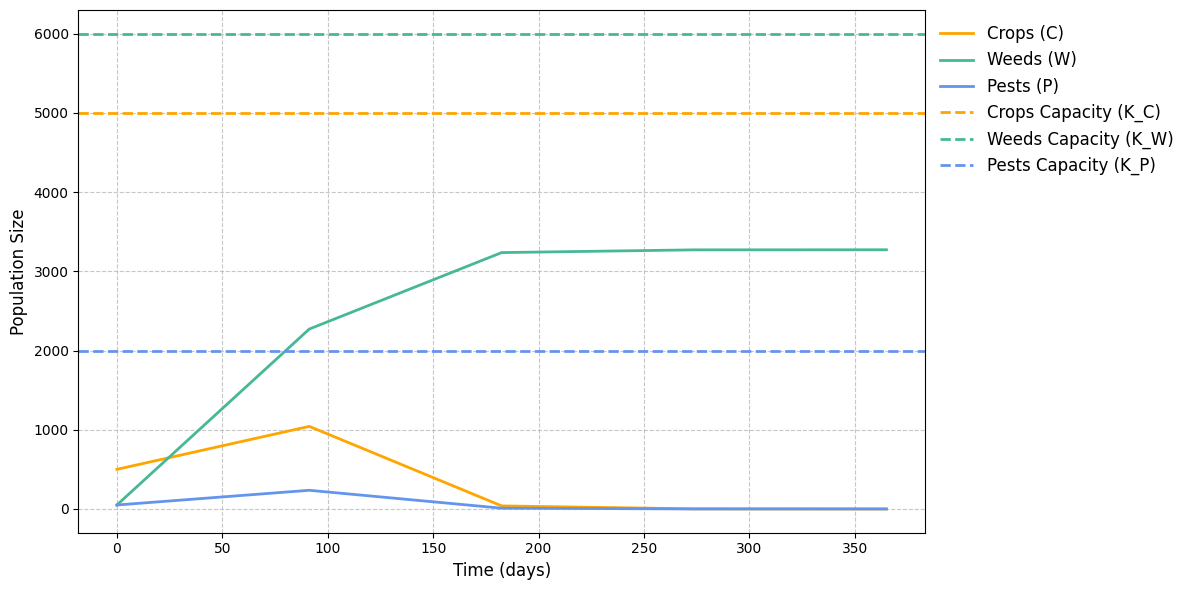
\includegraphics[width=0.8\textwidth]{1_1(basic).png}
    \caption{The evolution of the farmland ecosystem under basic assumptions.}
    \label{fig:FarmModel-V0}
\end{figure}

In Figure\ref{fig:FarmModel-V0}, we can know that as 
time progresses, the crop population size first increases and 
then decreases, reaching a peak at around 100 days and then 
declining to a relatively low level, which is far below the 
environmental carrying - capacity of 5000. The weed population 
size steadily increases from 0, reaches around 3000 at about 150 
days, and then remains stable, without reaching the environmental 
carrying - capacity of 6000. The pest population size experiences 
a slight increase in the initial stage, then rapidly decreases to 
near 0 and remains stable, far below the environmental carrying - 
capacity of 2000. It can be seen that weeds have strong 
competitiveness, the pest control effect is good, and crop growth 
is somewhat restricted, which is also in line with our expectations.

\noindent \textbf{Analysis of FarmModel-V1}

In \ref{eq:FarmModel-V1},we have introduced the concept of regular 
application of pesticides, and pesticide volatilization, drug resistance
and seasonal growth rate. We show the simulation results in 
Figure\ref{fig:FarmModel-V1}.

\begin{figure}[h]
    \centering
    \begin{subfigure}[b]{.4\textwidth}
        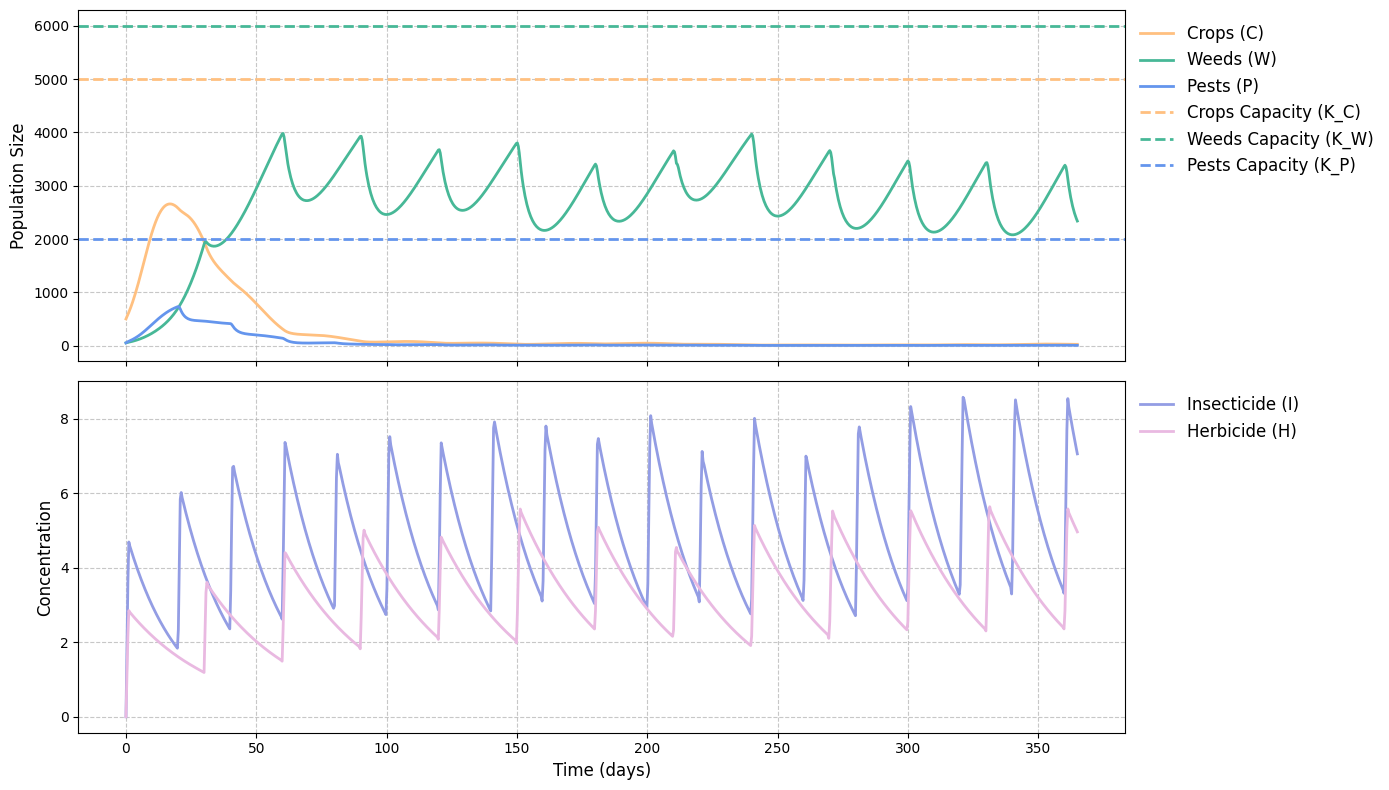
\includegraphics[width=\textwidth]{1_2(HI-pulse).png}
        \caption{HI-pulse}
    \end{subfigure}
    \begin{subfigure}[b]{.4\textwidth}
    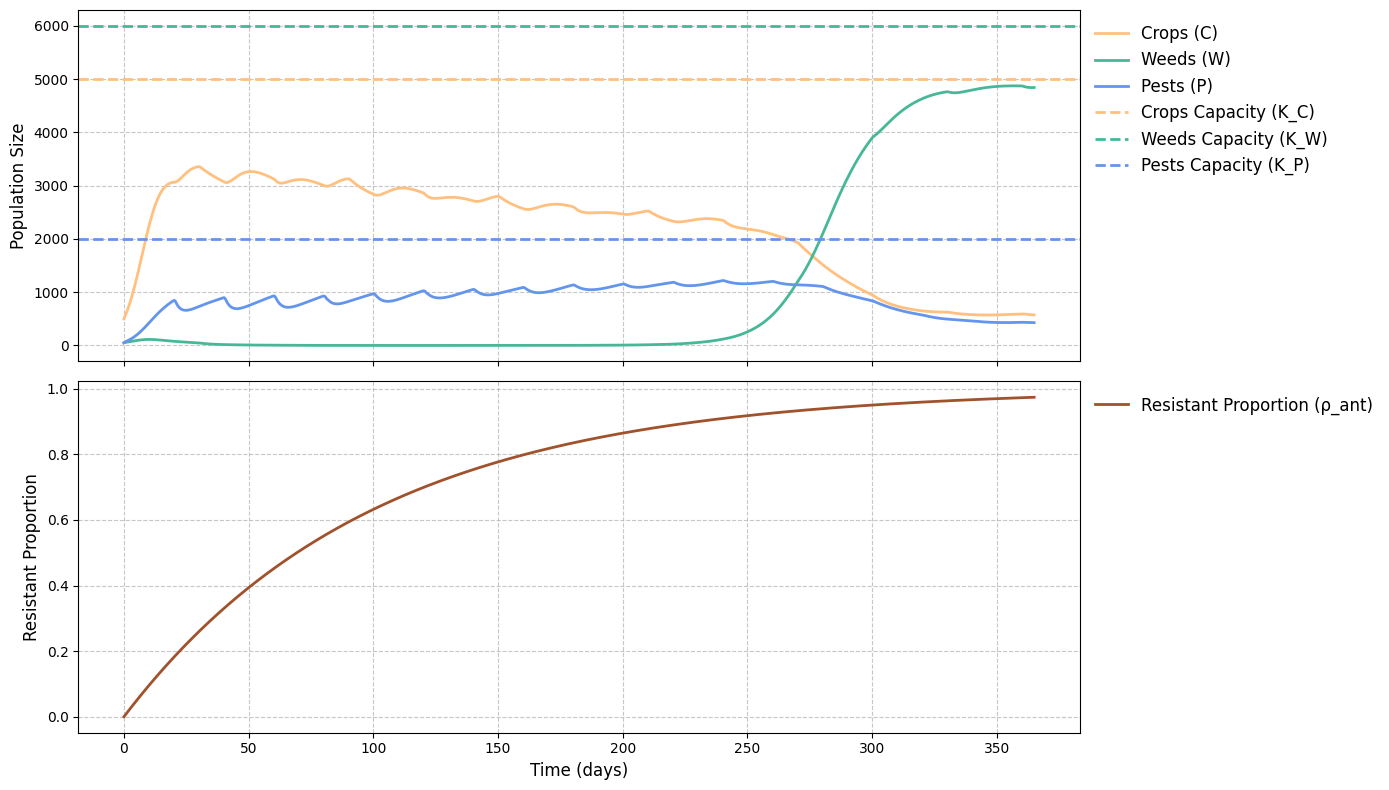
\includegraphics[width=\textwidth]{1_3(resist).png}
    \caption{Resist Effect}
    \end{subfigure}
    \begin{subfigure}[b]{.4\textwidth}
    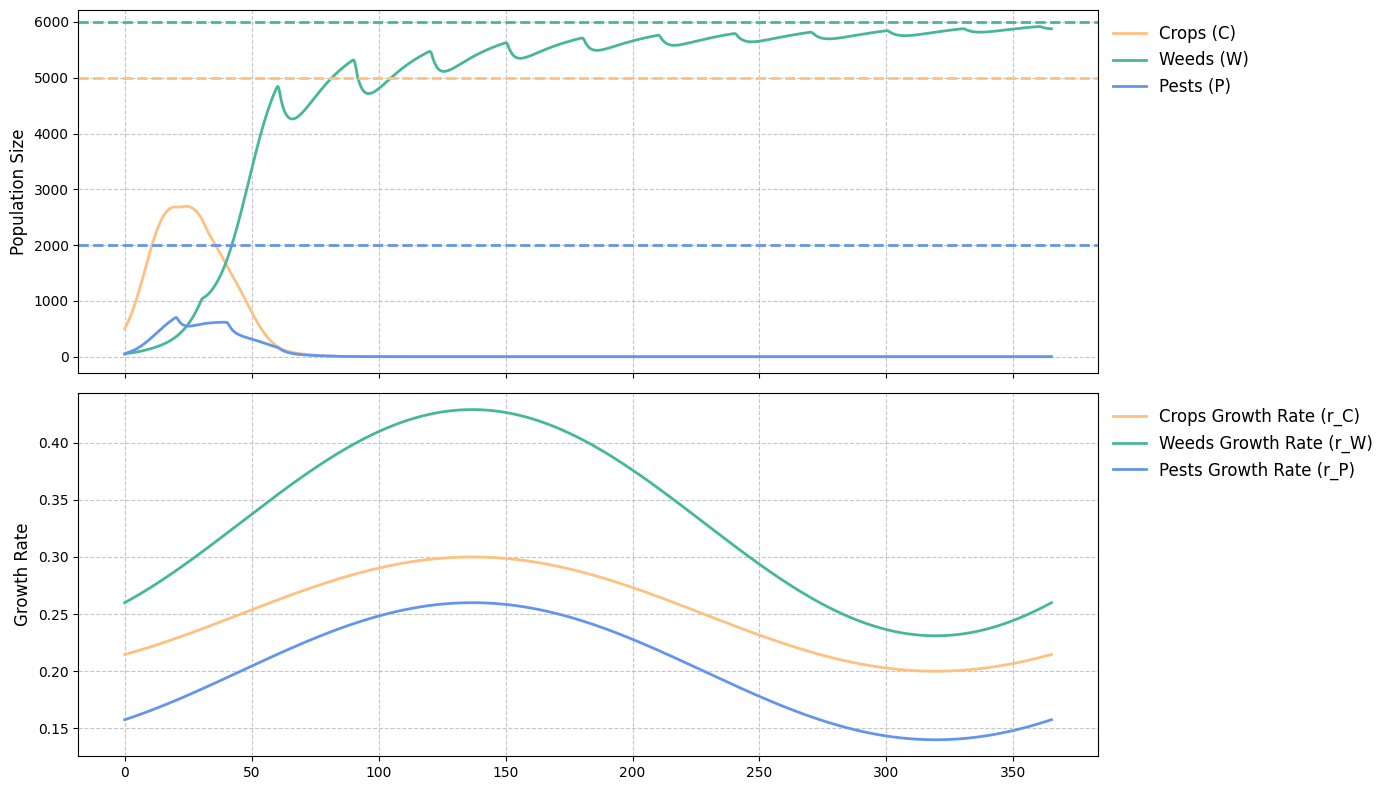
\includegraphics[width=\textwidth]{1_4(seasonal).png}
    \caption{Seasonal Variations}
    \end{subfigure}
    \begin{subfigure}[b]{.4\textwidth}
        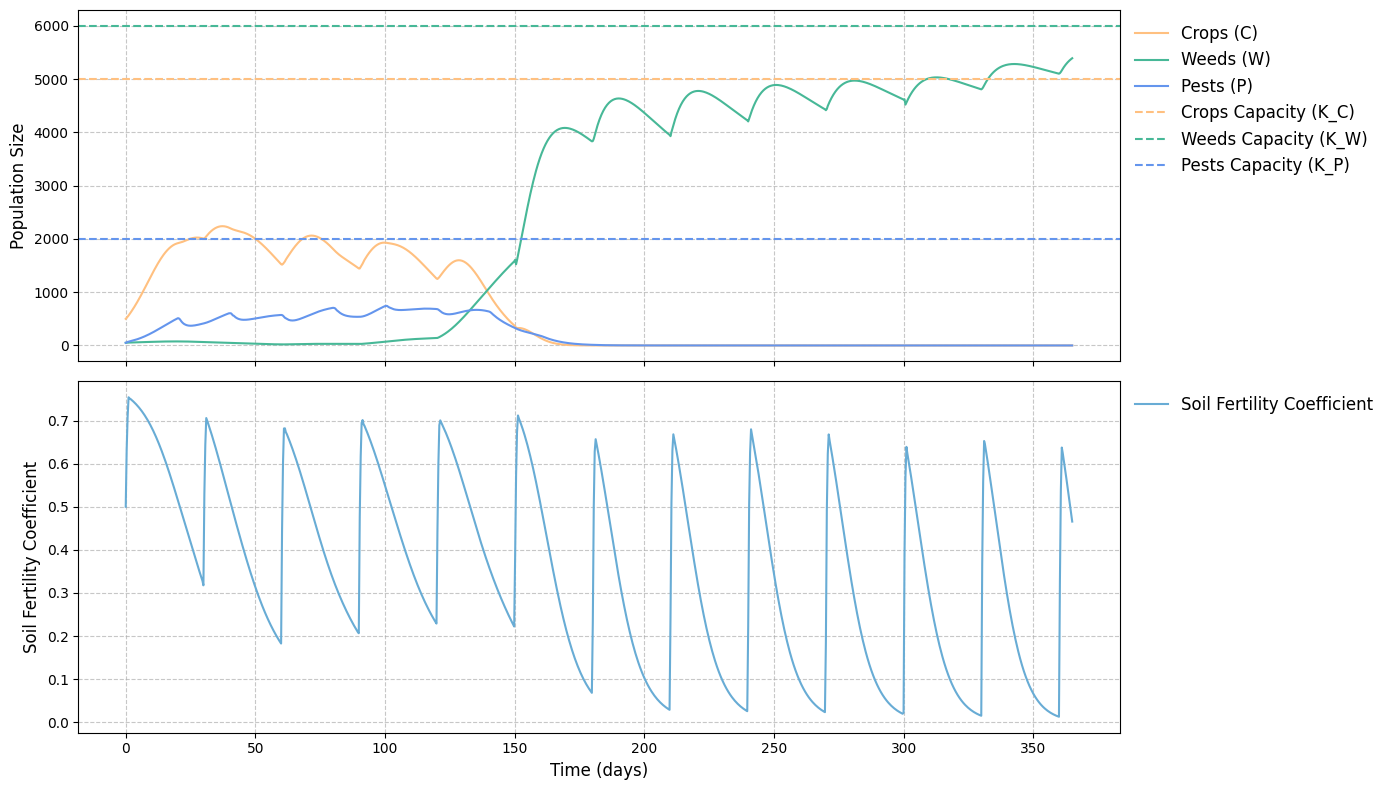
\includegraphics[width=\textwidth]{1_4(soil).png}
        \caption{Soil Variations}
    \end{subfigure}
    \caption{FarmModel-V1}\label{fig:FarmModel-V1}
    \end{figure}

    In (a), after the introduction of the pesticide pulse, the growth of crops 
    is initially inhibited, manifested as a change in their quantity growth 
    compared to the situation without the introduction. Nevertheless, the weed 
    quantity eventually dominates after fluctuations, which is related to the 
    pesticide volatilization. 
    The volatilization characteristics affect the duration and intensity of 
    the pesticide's effect. In (b), the crops initially show a 
    growth trend, but as the proportion of resistant individuals increases, their 
    growth is restricted, and the weeds dominate the system again, intuitively 
    reflecting the change in the competitive relationship between crops and weeds
     due to the resistance factor. (c) shows that under the influence
      of seasonal factors, the growth rates of crops and weeds fluctuate seasonally,
       yet the final dominance of weeds remains unchanged, indicating that although 
       seasonality has an impact, it is not a decisive factor. In (d), 
       the soil fertility coefficient fluctuates, reflecting the changes in soil 
       factors, but the growth trends of crops and weeds are still dominated by 
       weeds, indicating that the soil factor has a relatively limited impact on 
       the overall model.

\subsection{Task2: FarmModel-V2}
\subsubsection{Details about FarmModel-V2}
In this model, we introduce two species, BC and B, to represent the reemergence of species.

\noindent\textbf{Restoration of species BC}

BC represents a plant beneficial to the soil. In the farmland 
ecosystem, the restoration of species BC can improve soil conditions and 
increase soil fertility. Of course, we also need to take into account the 
competitive relationship between BC and other plants.

First, we calculate the growth rate of BC. The growth rate is same as \eqref{eq:seasonal1.0}
    , but we need add a scale factor and consider the gradual recovery of the basic growth rate:
    \begin{equation}
        \begin{aligned}
            r_{BC,0}(t) &= r_{BC,\text{max}} \cdot \left(1 - e^{-k_{BC} t}\right)\\
            r_{BC}(t) &= r_{BC,0} \cdot \left(1 + A_{BC} \cdot \sin\left(\frac{2\pi t}{365} + \phi_{BC}\right)\right) \cdot \frac{S}{K_S + S}
        \end{aligned}\label{eq:BC1.0}
    \end{equation}
    

And then we have the growth formula of BC:
    \begin{align}
        \frac{dBC}{dt} = BC \left[ r_{BC}(t) \left( 1 - \tilde{BC} \right) - \theta_{C,BC} \tilde{C} - \theta_{W,BC} \tilde{W} - \delta_{H,BC} \tilde{H} \right]\label{eq:BC1.1}
\end{align}

\noindent\textbf{Soil Fertility:} 

Considering the impacts of BC, C, and W on soil fertility, as well as the practice of regular fertilization, 
we have this formula for soil fertility:
\begin{equation}
    \begin{aligned}
        \frac{dS}{dt} &= S(\kappa_{BC} \tilde{BC} -\kappa_C \tilde{C} - \kappa_W \tilde{W} )\\
        S(t^+) &= S(t^-) + Q_S
    \end{aligned}\label{eq:soil1.0}
\end{equation}
The meanings of parameters are provided in the previous text.

\noindent\textbf{Restoration of species A}

In our setting, A is an organism that feeds solely on weeds. 
The restoration of its species has a certain inhibitory effect on weeds.
And we have:
\begin{align}
    r_{A,0}(t) &= r_{A,\text{max}} \cdot \left(1 - e^{-k_A t}\right)\\
    r_A(t) &= r_{A0} \cdot \left(1 + A_A \cdot \sin\left(\frac{2\pi t}{365} + \phi_A\right)\right) \label{eq:A1.0} \\
    \frac{dA}{dt} &= A \left[ r_A(t) \left( 1 - \tilde{A} \right) \cdot \beta_{WA} \cdot \frac{\tilde{W}}{\tilde{A}} - \delta_{HA} \tilde{H} \right]\label{eq:A1.1}
\end{align}

By synthesizing formulas \eqref{eq:BC1.0}\eqref{eq:BC1.1}\eqref{eq:soil1.0}\eqref{eq:A1.0}\eqref{eq:A1.1} and \eqref{eq:FarmModel-V1}, we can obtain \textbf{Farm
Model-V2}.

\subsubsection{Conclusion of FarmModel-V2}
In \textbf{FarmModel-V2}, we have the following conclusions:

\begin{enumerate}
    \item With the recovery of species, the numbers of BC 
    and A gradually increase from zero.
    \item After the introduction of BC and A, the 
    quantity of crops increased, and the number of 
    pests was controlled.
    \item As time changes, the populations of various 
    species exhibit stable cyclical fluctuations.
\end{enumerate}

\begin{figure}[h]
    \centering
    \begin{subfigure}[b]{.4\textwidth}
        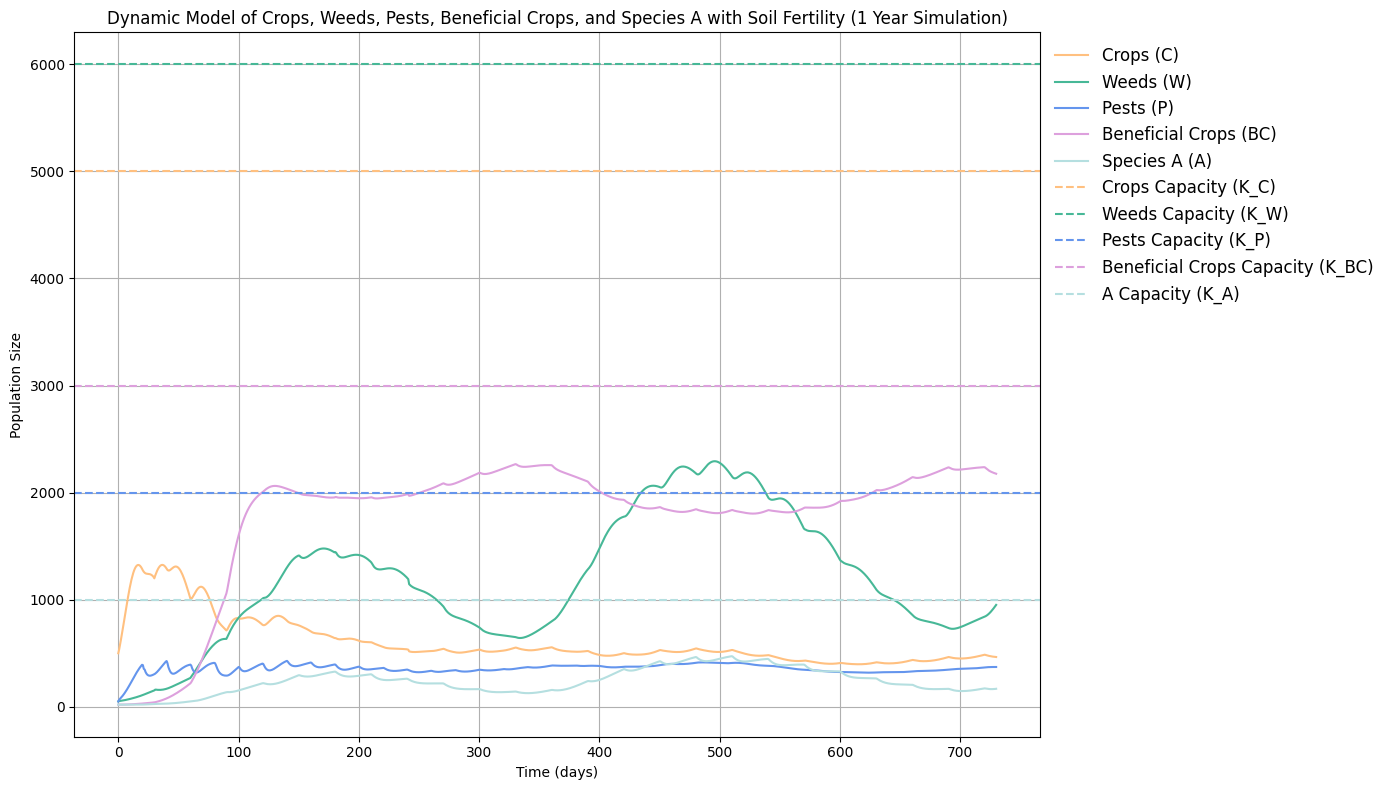
\includegraphics[width=\textwidth]{2_2(2years).png}
        \label{subfigure:2-2(2years)}
    \end{subfigure}
    \begin{subfigure}[b]{.4\textwidth}
        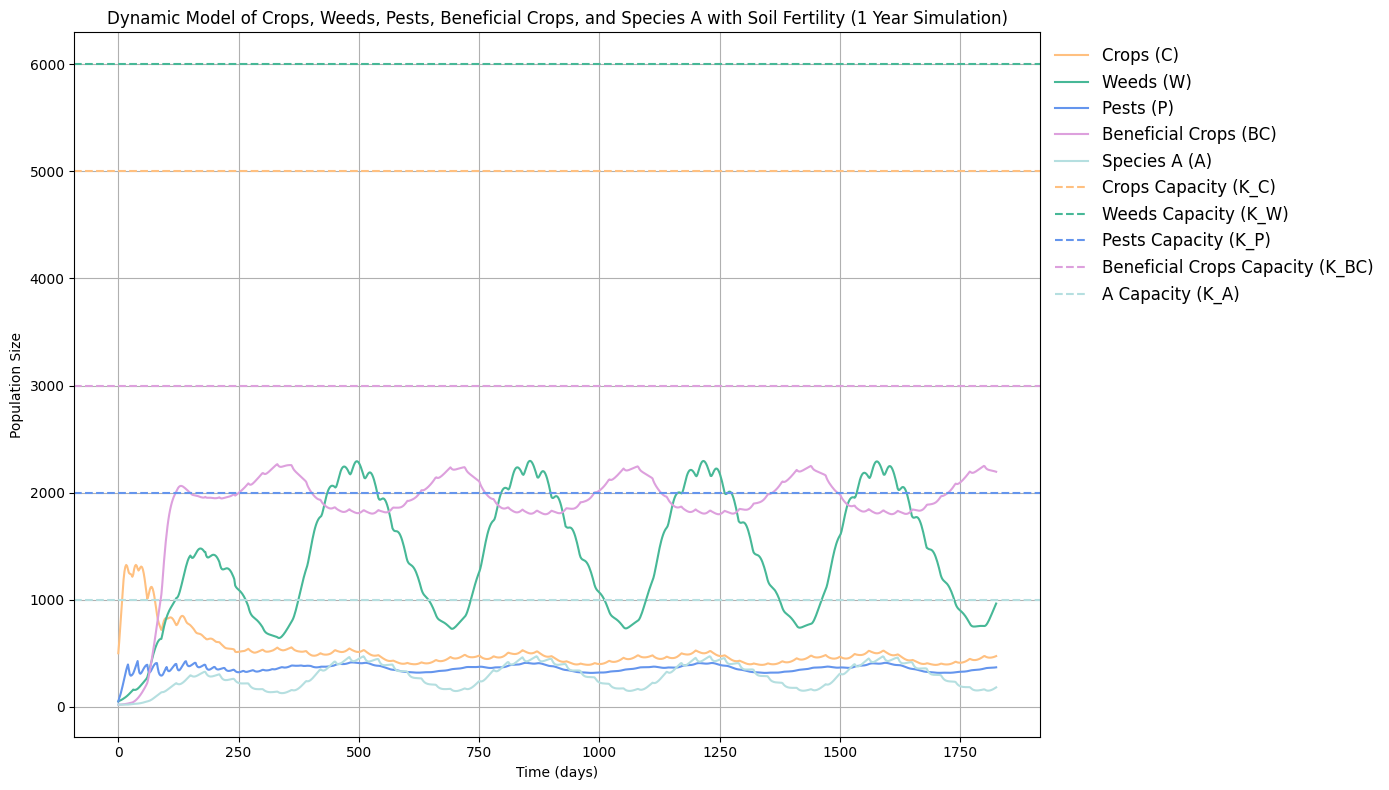
\includegraphics[width=\textwidth]{2_2(5years).png}
        \label{subfig:2-2(5years)}
    \end{subfigure}
    \caption{FarmModel-V2}\label{fig:FarmModel-V2}
    \end{figure}


\subsection{Task3: FarmModel-V3}
\subsubsection{Details about FarmModel-V3}
In this model, We 
attempt to remove the effects of pesticides in \ref{eq:FarmModel-V2} to
observe how the ecosystem would change under this condition. And then,
we introduce the concept of organic farming by incorporating organisms
such as bats and bees to regulate the balance of the ecosystem. 
As is well-known, bats can eat pests and weeds, while bees 
contribute to the pollination of crops.
By modeling
the interactions of these introduced species, we simulated the dynamics
among various variables, resulting in \textbf{FarmModel-V3}.

The model is nearly identical to the one in \textbf{FarmModel-V2}. 
In addition to introducing the factor of bat or bee, the pesticide formulas
 \eqref{eq:volatilization1} and \eqref{eq:volatilization2} have been remove.

\subsubsection{Conclusion of FarmModel-V3}
\noindent\textbf{Remove the effects of pesticides}

After removing the effects of pesticides, the ecosystem has changed 
significantly. The population of weeds has increased significantly,
and the population of crops has decreased significantly. And as
time progresses, the populations of various species maintain periodic oscillations.

\begin{figure}[h]
    \centering
    \begin{subfigure}[b]{.4\textwidth}
        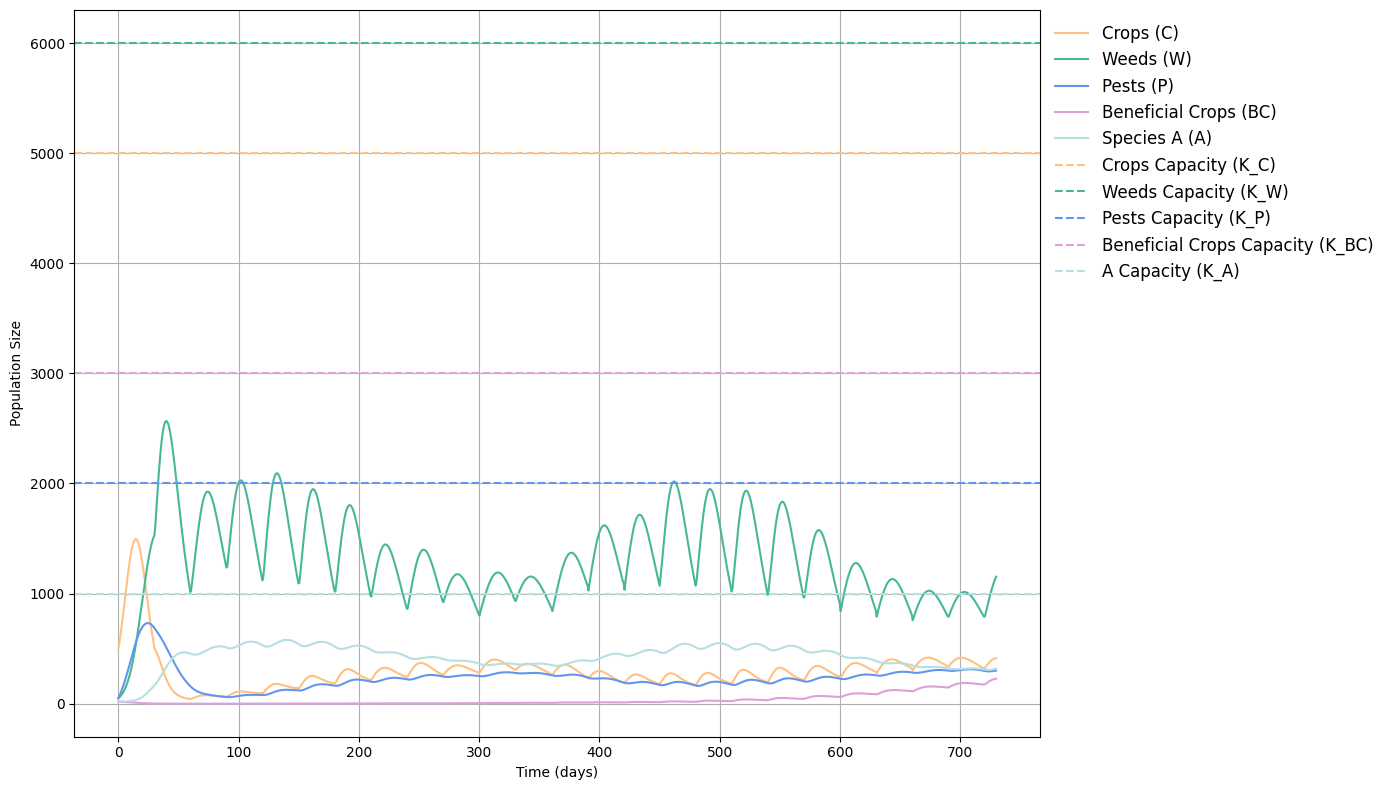
\includegraphics[width=\textwidth]{3_1(2years).png}
        \label{subfigure:3-1(2years)}
    \end{subfigure}
    \begin{subfigure}[b]{.4\textwidth}
        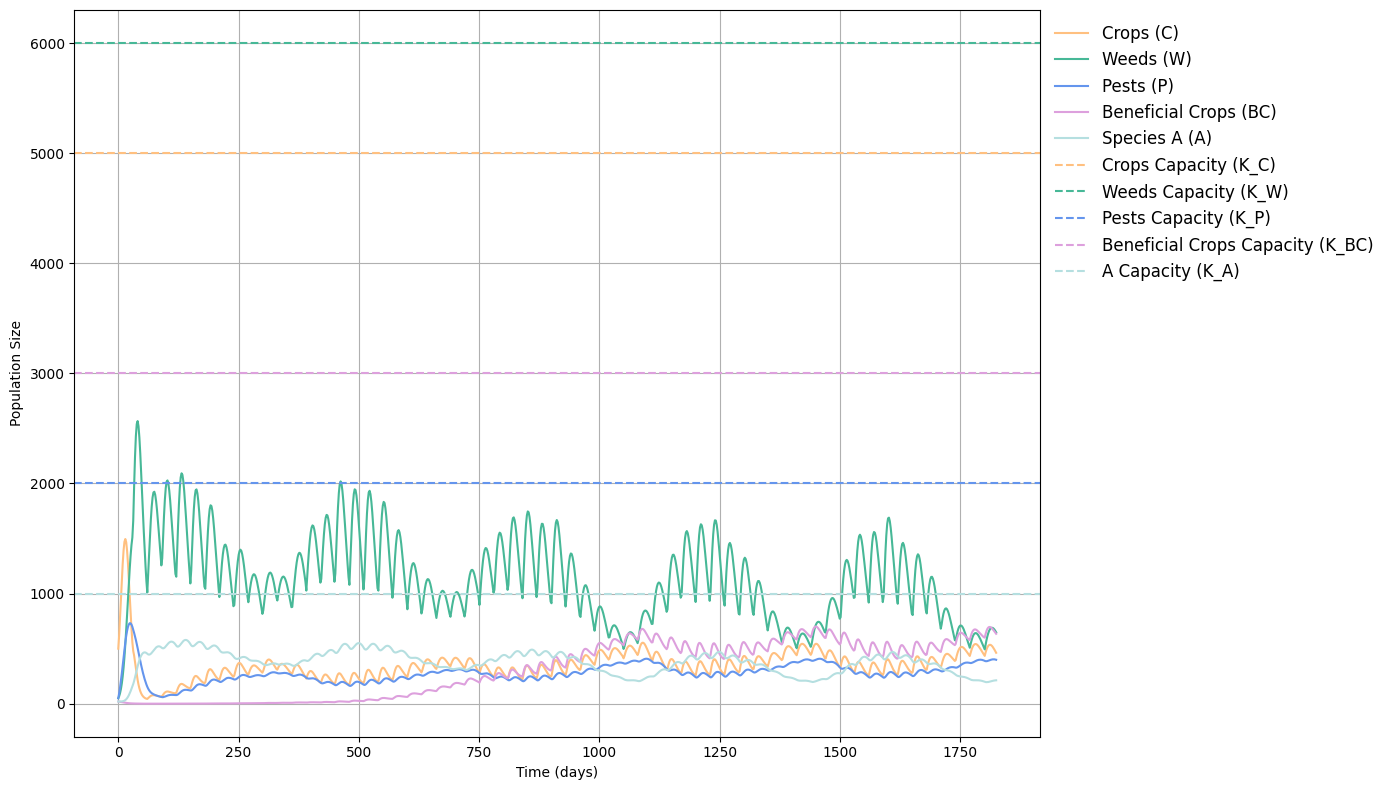
\includegraphics[width=\textwidth]{3_1(5years).png}
        \label{subfig:3-1(5years)}
    \end{subfigure}
    \caption{Remove Pesticides}\label{fig:FarmModel-V3.1}
    \end{figure}

\noindent\textbf{Introduce the concept of organic farming}

We introduced bats and bees respectively, and obtained the
 following results.

\begin{figure}[h]
    \centering
    \begin{subfigure}[b]{.4\textwidth}
        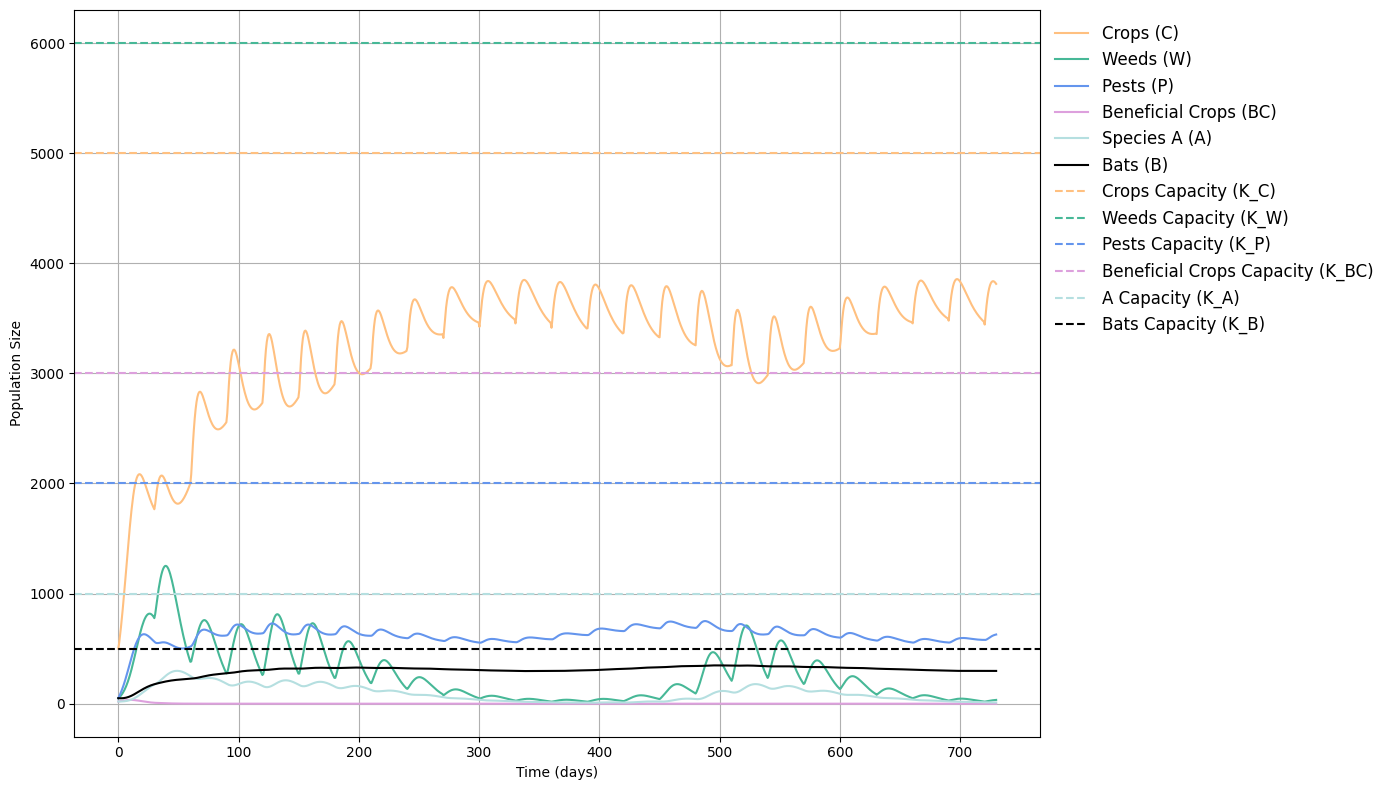
\includegraphics[width=\textwidth]{3_2(2years).png}
        \label{subfigure:3-2(2years)}
    \end{subfigure}
    \begin{subfigure}[b]{.4\textwidth}
        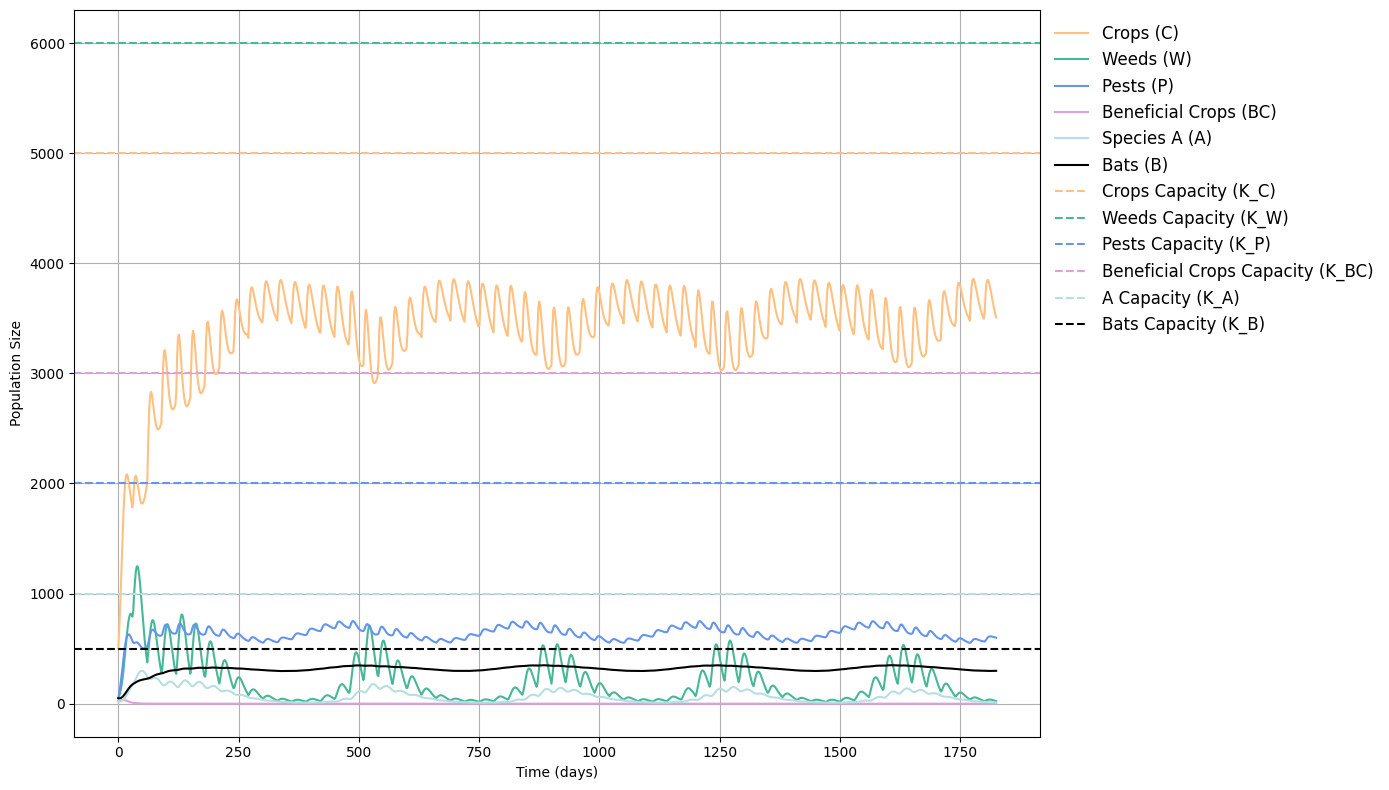
\includegraphics[width=\textwidth]{3_2(5years).png}
        \label{subfig:3-2(5years)}
    \end{subfigure}
    \caption{Introduce Bat}\label{fig:FarmModel-V3.2}
    \end{figure}

\begin{figure}[h]
    \centering
    \begin{subfigure}[b]{.4\textwidth}
        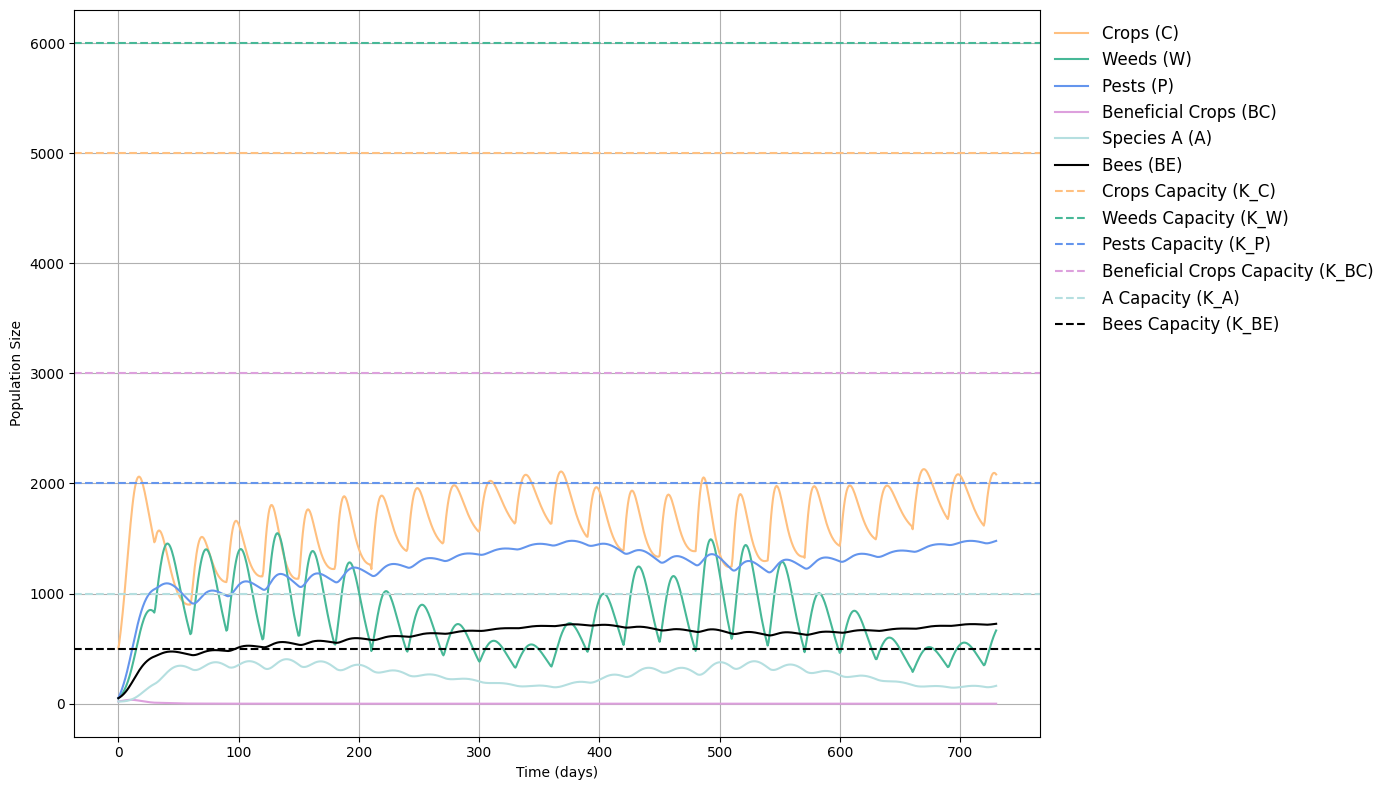
\includegraphics[width=\textwidth]{3_3(2years).png}
        \label{subfigure:3-3(2years)}
    \end{subfigure}
    \begin{subfigure}[b]{.4\textwidth}
        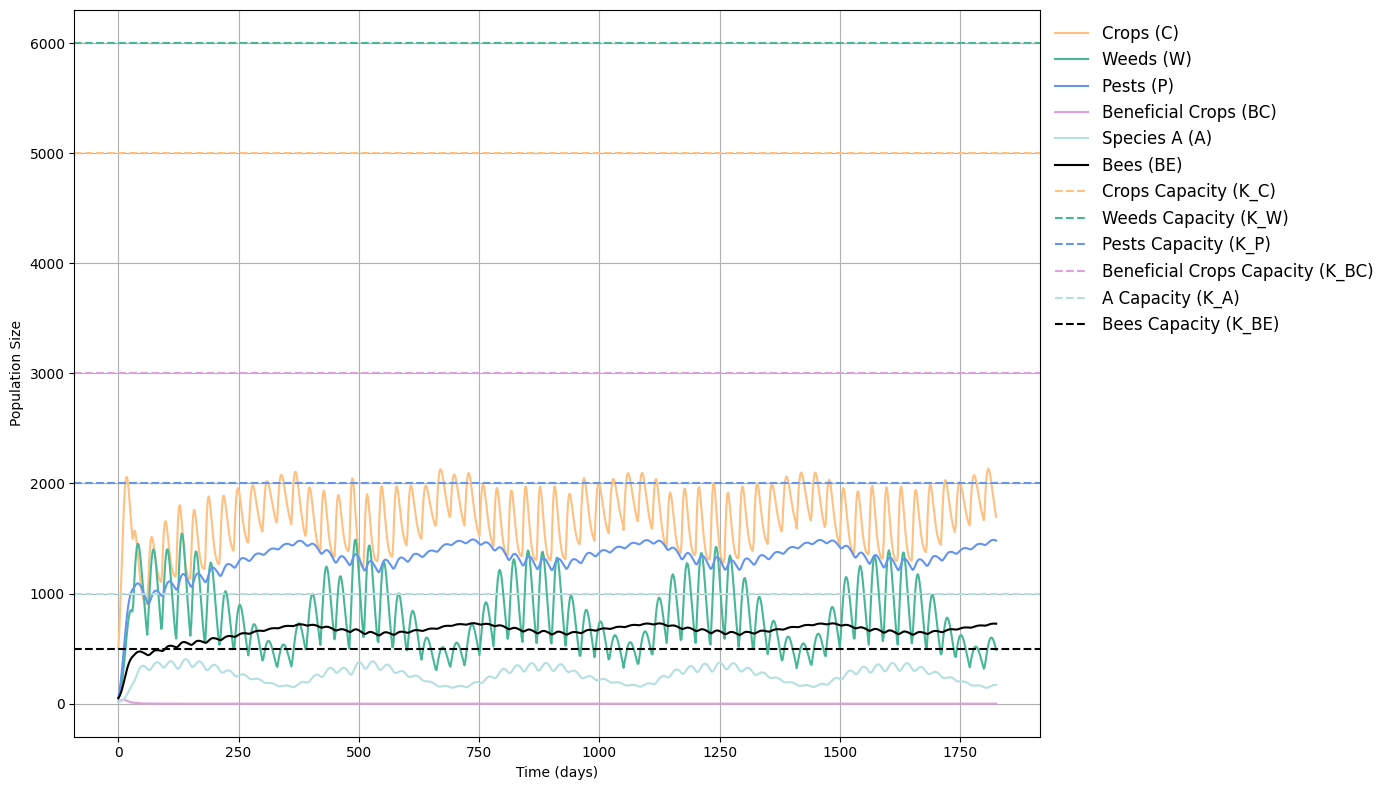
\includegraphics[width=\textwidth]{3_3(5years).png}
        \label{subfig:3-3(5years)}
    \end{subfigure}
    \caption{Introduce Bee}\label{fig:FarmModel-V3.3}
    \end{figure}

From Figure\ref{fig:FarmModel-V3.2} and 
Figure\ref{fig:FarmModel-V3.3}, we can see that the 
introduction of bats and bees has a significant impact 
on the ecosystem. The population of pests has been 
effectively controlled, and the population of crops 
has increased significantly. The population of weeds 
has also decreased significantly.

While we can also find that the bat has a better
control effect on pests and a better promote effect on 
crop than the bee.

\subsection{Task4: Go Green}
By reviewing the literature, we have summarized some green ecological 
evaluation indicators, as shown in the figure\ref{fig:Green Ecological Evaluation Indicators} below.

\begin{figure}[h]
    \centering
    
\includegraphics[width=0.4\textwidth]{image.png}
    \caption{Green Ecological Evaluation Indicators}
    \label{fig:Green Ecological Evaluation Indicators}
\end{figure}

We collect historical data from official websites such as GBIF (Global Biodiversity Information Facility) and FAO (Food and Agriculture Organization of the United Nations). By using the entropy - weight method, the weight of each indicator can be determined as $\omega_i$, which represents the angle of each part. The calculated GAI is:
\begin{equation}
\text{GAI}=(\omega_1\text{OM}+\omega_2\text{MC})+(\omega_3\text{NL}+\omega_4\text{PL})+(\omega_5\text{CDC}+\omega_6\text{AC})+\omega_7\text{SR}
\end{equation}

\subsubsection{Methods of Organic Farming}
Generally, the approaches to achieve organic agriculture are as followed:
\begin{enumerate}
    \item Using organic fertilizers.
    \item Adopting new planting methods, such as intercropping.
    \item Applying biological methods to kill pests instead of pesticides.
\end{enumerate}

\noindent{\textbf{Using Organic Fertilizers}}

When organic fertilizers are used, the organic matter and microbial content in the soil generally increase. Thus the change in GAI can be expressed as:

\begin{equation}
\Delta\text{GAI}_1 = \omega_1 \Delta\text{OM} + \omega_2 \Delta\text{MC}
\end{equation}

Where:
\begin{itemize}
    \item $\Delta\text{OM}$: Increase in organic matter
    \item $\Delta\text{MC}$: Increase in microbial content
\end{itemize}

\noindent{\textbf{Adopting New Planting Methods}}

Changing traditional planting methods allows for mutual nutrient supplementation between different crops. It can increase inorganic salts in the aquatic environment. At the same time, the space is fully utilized. This ensures sufficient air and allows for more compounds such as carbon dioxide, which benefits crop growth. Thus the change in GAI can be expressed as:

\begin{equation}
\Delta\text{GAI}_2 = \omega_3 \Delta\text{NL} + \omega_4 \Delta\text{PL} + \omega_5 \Delta\text{CDC} + \omega_6 \Delta\text{AC}
\end{equation}

\noindent{\textbf{Applying Biological Methods}}

Organic agriculture emphasizes environmental protection. It avoids chemical pesticides and utilizes biological methods to control pests. For example, when planting corn, Trichogramma are used to manage Ostrinia furnacalis. This enhances biodiversity. Compared with chemical pesticides, biological control avoids soil damage and helps maintain the activity of soil microbes. Thus the change in GAI can be expressed as:

\begin{equation}
\Delta\text{GAI}_3 = \omega_7 \Delta\text{SR} + \omega_1 \Delta\text{OM} + \omega_2 \Delta\text{MC}
\end{equation}

Therefore, the overall impact on the whole ecosystem is expressed as:

\begin{equation}
\Delta\text{GAI} = \Delta\text{GAI}_1 \times I_{\text{method1}} + \Delta\text{GAI}_2 \times I_{\text{method2}} + \Delta\text{GAI}_3 \times I_{\text{method3}}
\end{equation}

Where:
\begin{itemize}
    \item $I_{\text{method}}$ represents the Indicator Function of each method.
\end{itemize}

To sum up, organic fertilizer can improve the quality of soil. New planting methods have impacts on the aquatic environment and air, while biological methods can also improve the soil and increase biodiversity as well. The overall impact to the ecosystem is reflected on the change in GAI.

\subsubsection{Discussion of Costs and Benefits}
\noindent{\textbf{Costs}}

Agriculture, as the primary industry, has a significant impact on human’s life. Some advocate for the full implementation of active policies, promoting green agriculture comprehensively, while others emphasize adopting strategies based on local circumstances. The price of organic farming equipment is always much higher than conventional pesticides, which increases costs to some extent. For impoverished areas, it is particularly challenging for farmers to implement organic agriculture. Evaluating agricultural development in such regions using the Green Agriculture Index may not be a proper choice.

\noindent{\textbf{Benefits}}
\begin{enumerate}
    \item \textbf{Sustainable Productivity}
    
    Green agriculture helps maintain long-term ecological balance, contributing to the sustainable productivity of agriculture. Although initial investments may lead to short-term profit declines, improving the growing environment for crops can achieve steady growth in agricultural productivity over the long run. This, in return, enhances yields and increases income.
    \item \textbf{Moderate Change}
    
    Green agriculture still aims to improve agricultural yields. Thus, most regions do not need great adjustments to achieve sustainability while developing organic farming. This can avoid significant disruptions to farmlands, thereby preventing losses and ensuring the stability of the industry at the same time.

    \end{enumerate}
    \noindent\textbf{Simulation of Cost and Revenue}
    
    It is without doubt that the initial purpose of farming is to generate profit. So we take the cost and revenue into our consideration. Thus we can make comparisons between green agriculture and traditional agriculture on the aspect of economy.

    To calculate the farmers' profit, we collect data on crop prices, pesticide prices, etc., from the market, and simulate crop yields through differential equations under  different conditions . Here, we make comparisons between introducing a new species (we take bats as example) and using pesticide and herbicide.

    We used Monte Carlo simulation to model the different growth rates of crops and weeds. Based on the simulated data, we calculated the costs and revenues. Clearly, not every simulated scenario reflects the real situation. Since ecosystems transitioning from forests to farmland are always large-scale, we consider simulations with costs (or revenues) under 100 as invalid and exclude them from consideration.
    \begin{figure}[h]
        \centering
        \begin{subfigure}[b]{.4\textwidth}
            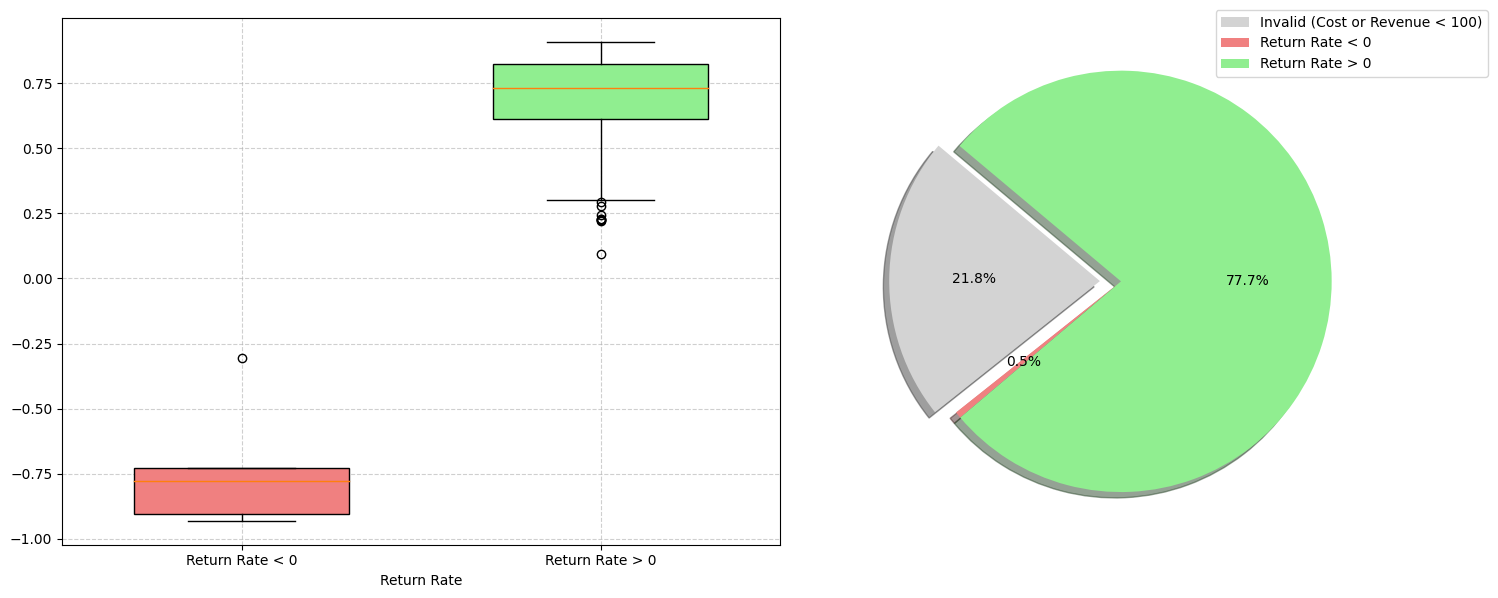
\includegraphics[width=\textwidth]{image1.png}
        \end{subfigure}
        \begin{subfigure}[b]{.4\textwidth}
            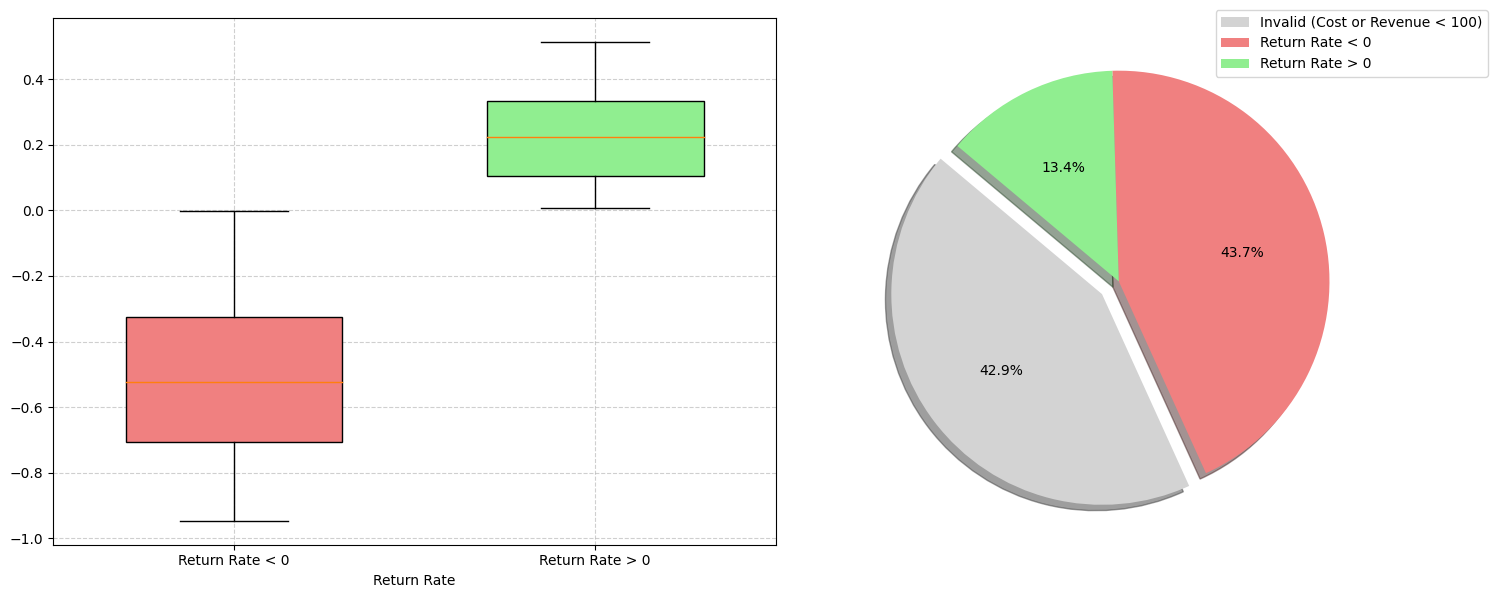
\includegraphics[width=\textwidth]{image2.png}
        \end{subfigure}
    \end{figure}

    As the charts above show, when introducing bats, the likelihood of positive expected profits is much higher than using pesticides. Furthermore, in cases where profits are positive, the return rate is also higher. The results mean that introducing bats offers a better profit expectation.
    \begin{figure}[h]
        \centering
        \begin{subfigure}[b]{.4\textwidth}
            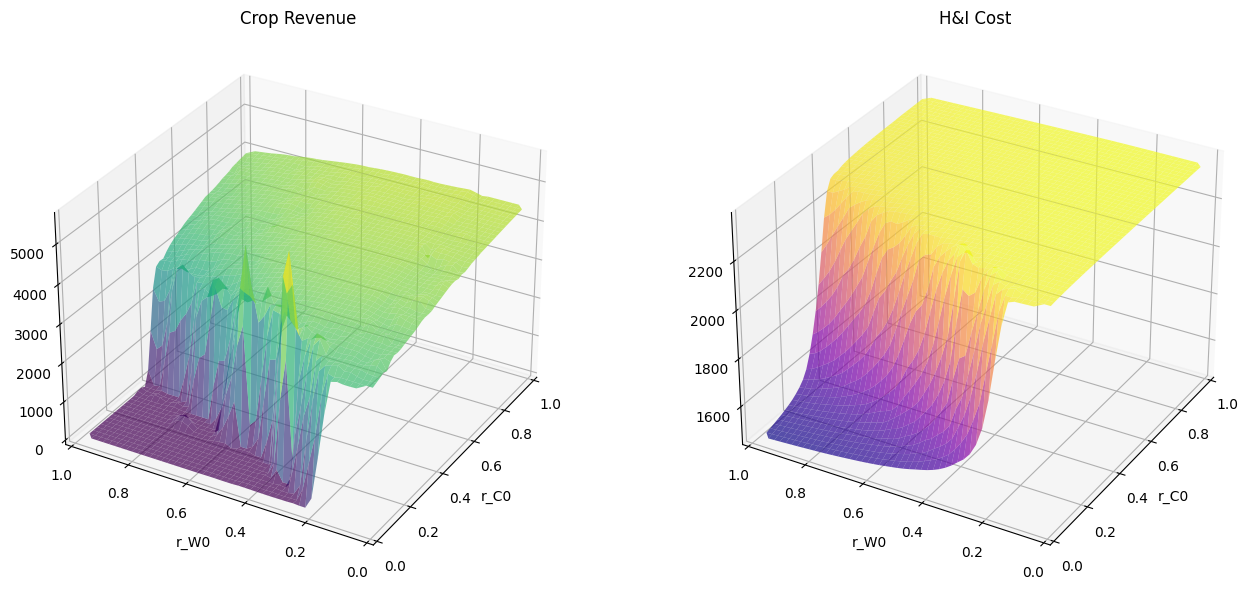
\includegraphics[width=\textwidth]{image3.png}
        \end{subfigure}
        \begin{subfigure}[b]{.4\textwidth}
            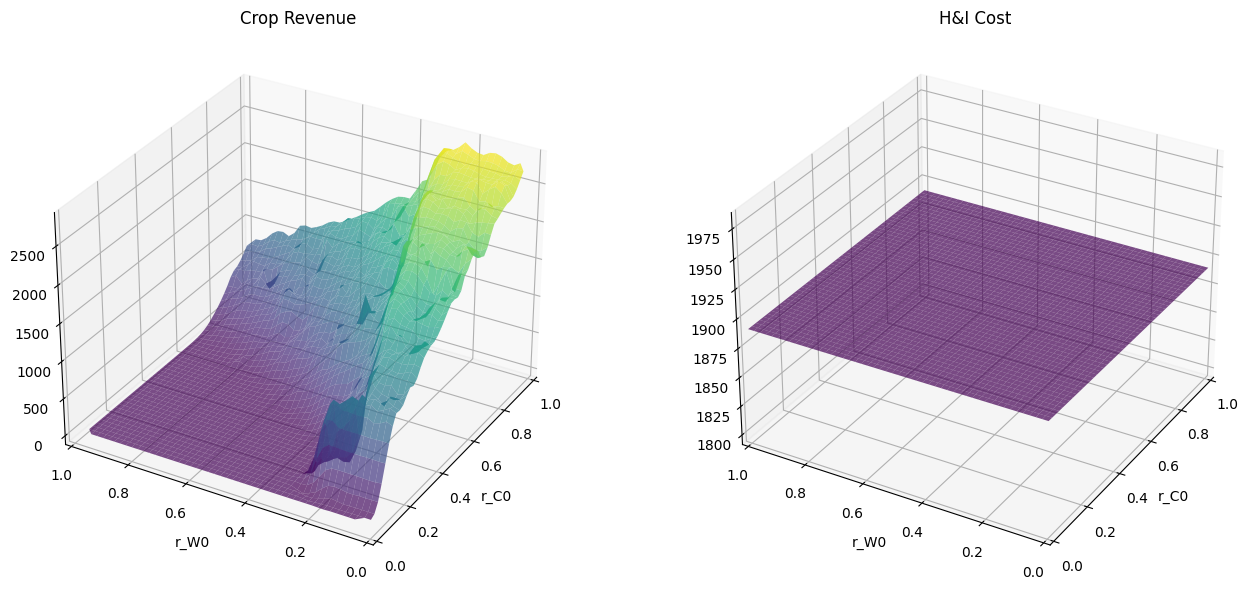
\includegraphics[width=\textwidth]{image4.png}
        \end{subfigure}
    \end{figure}

    The 3D plot provides a more clear view of the revenue and cost under various scenarios. When introducing bats, the costs are more likely to be higher than those when using pesticides. In the revenue plot of introducing bats, the larger area at high level represents a greater likelihood of obtaining higher revenue.

    Overall, introducing bats shows promising profit potential, with lower risks and higher stability. And compared to using pesticides, it is also more environmentally friendly. In this simulation, it is clear that adopting organic farming has more advantages.




\section{Evaluation and Analysis}

\subsection{Disaster Resilience: FarmModel-V3$_{\alpha,\beta,\gamma}$}
To evaluate the stability of these ecosystems (i.e., 
their resilience to natural disasters) and provide planting 
recommendations based on the agricultural ecosystem, 
we developed the \textbf{FarmModel-V3$_{\alpha,\beta,\gamma}$}.

\subsubsection{Drought: FarmModel-V3$_{\alpha}$}
Let the occurrence time point be $t_0$ and the duration be $T_D$.
During the drought period, the growth rates of crops, 
weeds, and pests,$r_C$, $r_W$, and $r_P$ are severely negatively impacted. 
After the drought ends, the growth rates gradually recover (let it be $\lambda_D$), so we have:

\noindent{\textbf{Growth Rate:}}
\begin{equation}
    \begin{aligned}
    r_{\mathcal X}(t) = 
    \begin{cases} 
    r_{\mathcal X} \cdot (1 - Disas_D) & \text{if } t_0 \leq t < t_0 + T_D \\
    r_{\mathcal X} \cdot \left(1 - Disas_D \cdot e^{-\lambda_D (t - t_0 - T_D)}\right) & \text{if } t \geq t_0 + T_D
    \end{cases}
    \end{aligned}\label{eq:growth-rate-drought}
\end{equation}
Here: $\mathcal X$ can be $C$, $W$, or $P$.

By using \eqref{eq:growth-rate-drought} and \eqref{eq:crop1.0}\eqref{eq:weed1.0}\eqref{eq:pest1.0}
to modify \textbf{FarmModel-V$3$}, we can obtain \textbf{FarmModel-V3$_{\alpha}$}.
\begin{figure}
    \centering
    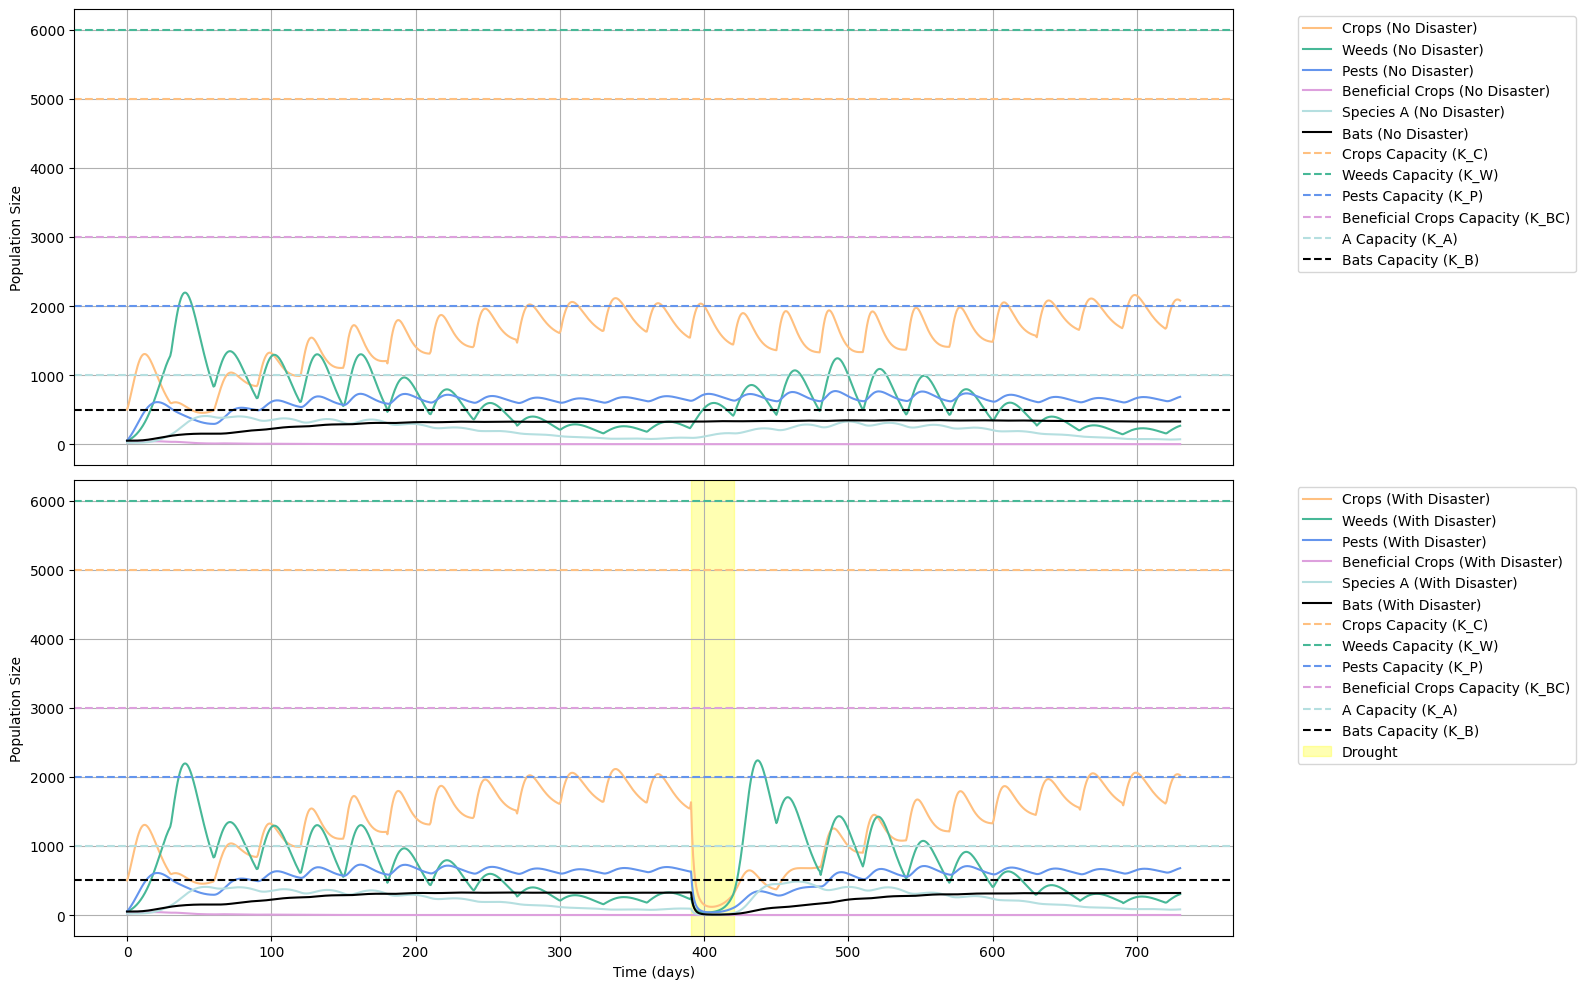
\includegraphics[width=0.8\textwidth]{drought(2years).png}
    \caption{The evolution of the farmland ecosystem under drought conditions.}
    \label{fig:Drought Influence}
\end{figure}
In Figure\ref{fig:Drought Influence}, we can see that 
after the drought occurred (marked in yellow), the populations 
of various organisms dropped abruptly.After that, the weeds 
recovered significantly first. Subsequently, other species 
gradually restored and returned to their original states, 
thus reverting to a stable ecosystem.


\subsubsection{Flood: FarmModel-V3$_{\beta}$}
Let the occurrence time point be $t_0$ and the duration be $T_F$.Unlike 
droughts, when flood disasters occur, we assume that the quantities of 
crops, weeds, and pests will decrease suddenly in proportion, and their 
growth rates will also be severely impacted. After the floods end, the 
growth rates gradually recover.Based on these assumptions, we have
\textbf{FarmModel-V3$_{\beta}$}:

\noindent{\textbf{Growth Rate:}}
\begin{equation}
    \begin{aligned}
    r_{\mathcal X}(t) = 
    \begin{cases} 
    r_{\mathcal X} \cdot (1 - Disas_F) & \text{if } t_0 \leq t < t_0 + T_F \\
    r_{\mathcal X} \cdot \left(1 - Disas_F \cdot e^{-\lambda_F (t - t_0 - T_F)}\right) & \text{if } t \geq t_0 + T_F
    \end{cases}
    \end{aligned}\label{eq:growth-rate-flood}
\end{equation}
Here: $\mathcal X$ can be $C$, $W$, or $P$.

\noindent{\textbf{Crop:}}
\begin{equation}
    \begin{aligned}
    C(t_0^+) = C(t_0^-) \cdot (1 - \gamma_F \cdot Disas_F)
    \end{aligned}\label{eq:flood-C}
\end{equation}

\noindent{\textbf{Weed:}}
\begin{equation}
    \begin{aligned}
    W(t_0^+) = W(t_0^-) \cdot (1 - \gamma_F \cdot Disas_F)
    \end{aligned}\label{eq:flood-W}
\end{equation}

\noindent{\textbf{Pest:}}
\begin{equation}
    \begin{aligned}
        P(t_0^+) = P(t_0^-) \cdot (1 - \gamma_F \cdot Disas_F)
    \end{aligned}\label{eq:flood-P}
\end{equation}

By using \eqref{eq:growth-rate-flood}\eqref{eq:flood-C}\eqref{eq:flood-P}
 and \eqref{eq:flood-W} to modify \textbf{FarmModel-V3}, we can obtain \textbf{FarmModel-V3$_{\beta}$}.

\begin{figure}
    \centering
    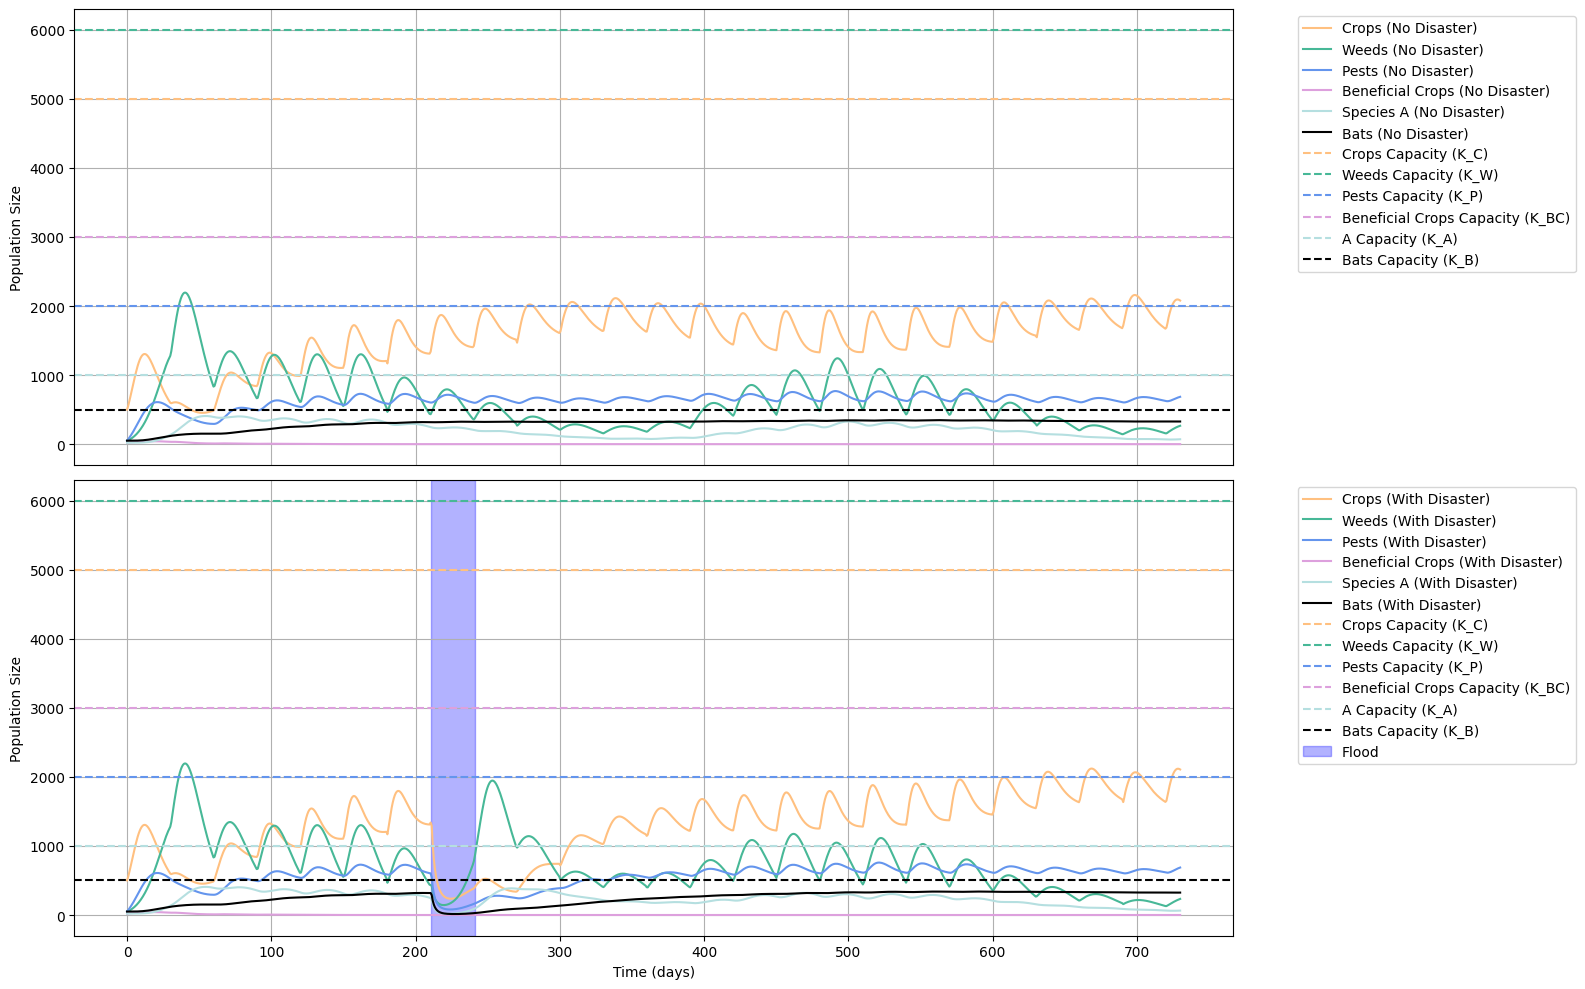
\includegraphics[width=0.8\textwidth]{flood(2years).png}
    \caption{The evolution of the farmland ecosystem under flood conditions.}
    \label{fig:Flood Influence}
\end{figure}

In Figure\ref{fig:Flood Influence}, we can see that The flood (marked 
in purple) had a more significant impact on reducing the quantity of 
various crops. However, compared to the drought, the recovery rate of 
each species was relatively faster after the disaster.

\subsubsection{Insect Plague: FarmModel-V3$_{\gamma}$}

Let the occurrence time point be $t_0$ and the duration be $T_I$. 
When insect plagues occur, the growth rates of pest will increase 
suddenly. After the insect plagues end, the growth rates gradually recover. 
That is:
\begin{equation}
    \begin{aligned}
        r_P(t) &= 
        \begin{cases} 
        r_P \cdot (1 + Disas_I) & \text{if } t_0 \leq t < t_0 + T_I \\
        r_P \cdot \left(1 + Disas_I \cdot e^{-\lambda_I (t - t_0 - T_I)}\right) & \text{if } t \geq t_0 + T_I
        \end{cases}\\
        \frac{dP}{dt} &= P \left[ r_P(t) \left( 1 - \frac{P}{K_P} \right) + \beta_{CP} \frac{C}{K_C} - \mu_{IP} I \right]
    \end{aligned}
\end{equation}

Base on the above analysis, we can obtain \textbf{FarmModel-V3$_{\gamma}$}.

From the simulation results in Figure\ref{fig:Insect Plague Influence}, we can 
see that the pest population size increased significantly during the insect
plague period (marked in red), and the populations of other species were
significantly reduced. After the insect plague ended, the populations of
various species gradually recovered, and the ecosystem returned to a stable state.

\begin{figure}[h]
    \centering
        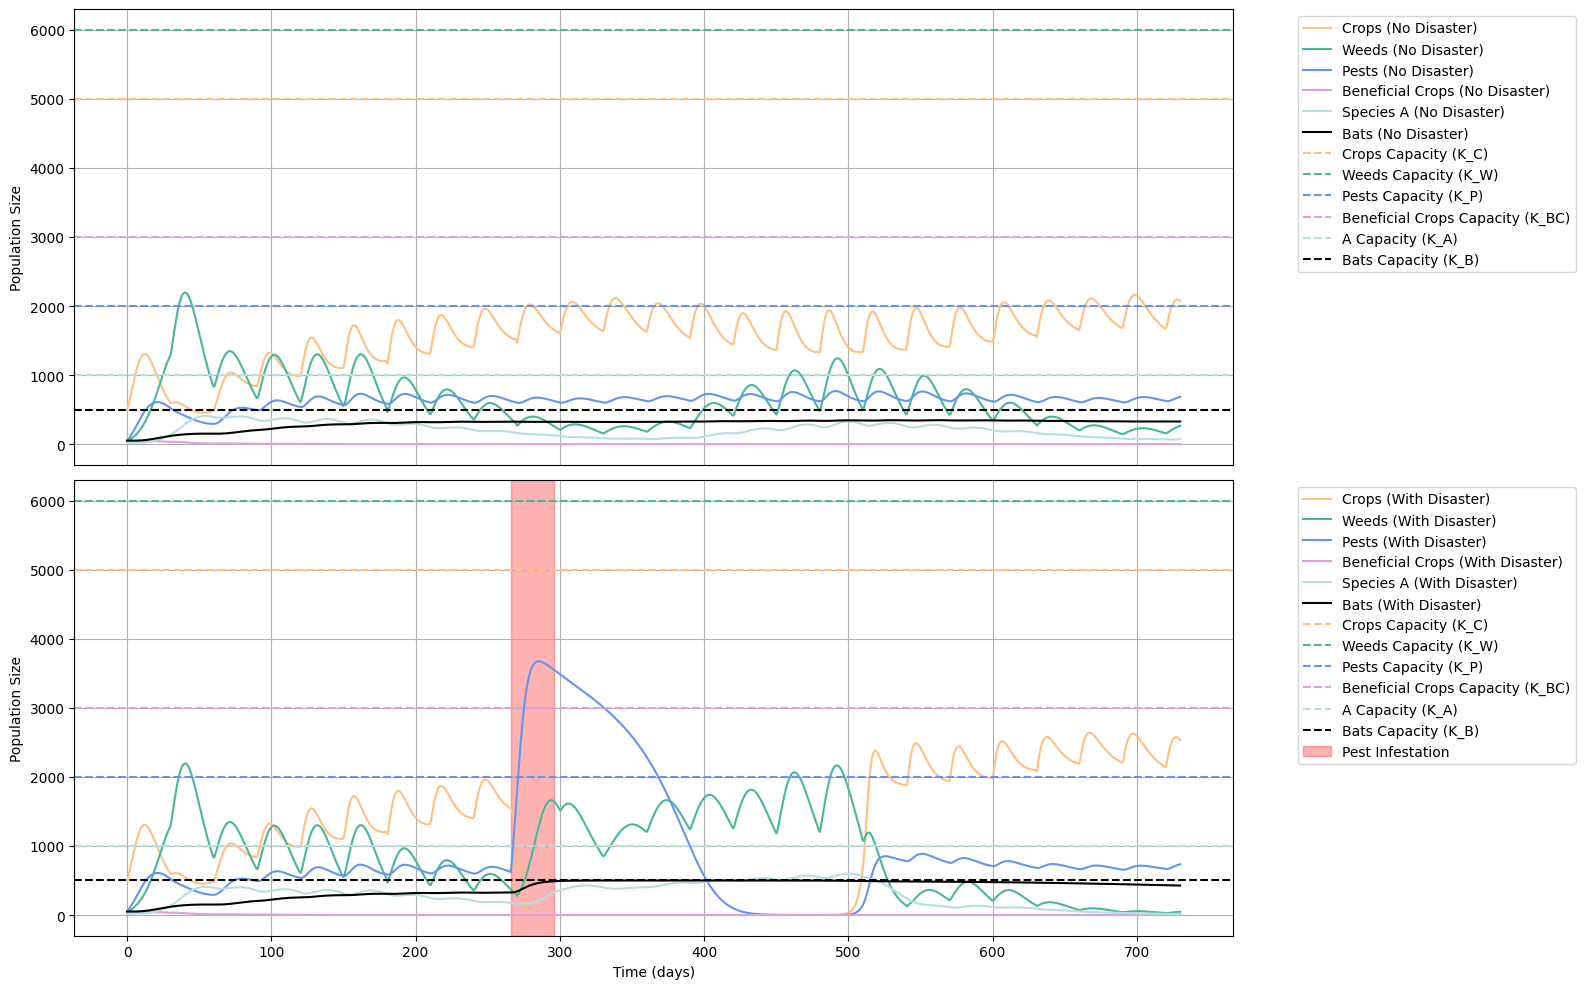
\includegraphics[width=0.8\textwidth]{pest(2years).png}
        \label{subfig:3-2(2years)}
    \caption{ The evolution of the farmland ecosystem under insect Plague}\label{fig:Insect Plague Influence}
    \end{figure}

\subsubsection{Conclusion of FarmModel-V3$_{\alpha,\beta,\gamma}$}
In the \textbf{FarmModel-V3$_{\alpha,\beta,\gamma}$}, we have the following conclusions:
\begin{enumerate}
    \item The ecosystem is relatively stable, and it can recover quickly after natural disasters.
    \item In the long run, FarmModel - V3 always maintains dynamic stability,
    and sudden natural disasters do not permanently alter the cycle of the
     ecosystem.
\end{enumerate}
    
\subsection{Sentivity Analysis: \textbf{\textcolor{red}{$\triangle$}Monte Carlo Simulation}}

\subsubsection{FarmModel-V1}
In this study, the Monte Carlo simulation method was used to conduct a simulation analysis of the quantity changes of crops (C), weeds (W), and pests (P) in the ecosystem. First, the basic growth rate of crops \(r_{C0}\) and the basic growth rate of weeds \(r_{W0}\) were selected as key parameters, and the value ranges of these two parameters are both \([0, 1]\). Then, 1000 simulation experiments with a duration of 1 year were carried out. In each simulation, the values of \(r_{C0}\) and \(r_{W0}\) were randomly generated, and the quantities of each species at the end of the simulation were calculated.

The reasons for selecting these two parameters are as follows:
\begin{enumerate}
    \item Parameter sensitivity: Through preliminary sensitivity analysis, we found that \(r_{C0}\) and \(r_{W0}\) are key variables affecting the quantity trends of crops and weeds. Changes in these parameters can significantly alter the interactions among species and the overall state of the ecosystem.
    
    \item  Important components of the ecosystem: Crops and weeds are two important components of the ecosystem. The growth of crops directly impacts agricultural yields, while the growth of weeds may exert competitive pressure on crops, thus affecting the stability and productivity of the ecosystem.
\end{enumerate}

Based on the simulation results, we plotted 3D graphs to show the relationship between the number of species and \(r_{C0}\) and \(r_{W0}\). By observing these 3D graphs, we found that the changes in the number of species exhibit distinct dividing surfaces under certain combinations of \(r_{C0}\) and \(r_{W0}\). These dividing surfaces are extremely steep, and their projections are generally in the shape of a straight line.

\begin{figure}[h]
    \centering
    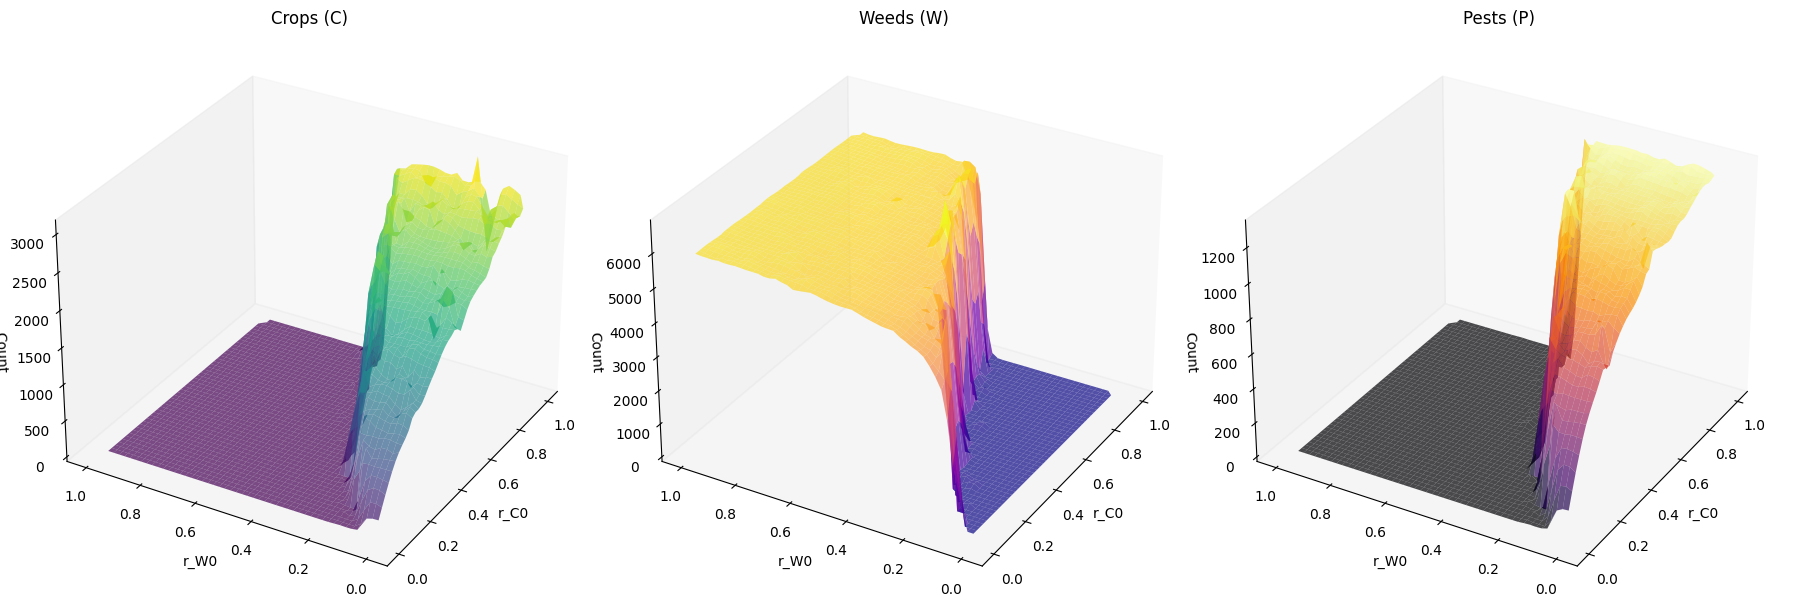
\includegraphics[width=0.8\textwidth]{m1-mk3D.png}
    \caption{3D:Monte Carlo of FarmModel-V1}
\end{figure}

To further analyze the dividing surfaces, we selected the points of the three species on the dividing boundaries and projected them onto a two - dimensional plane.

\begin{figure}[h]
    \centering
    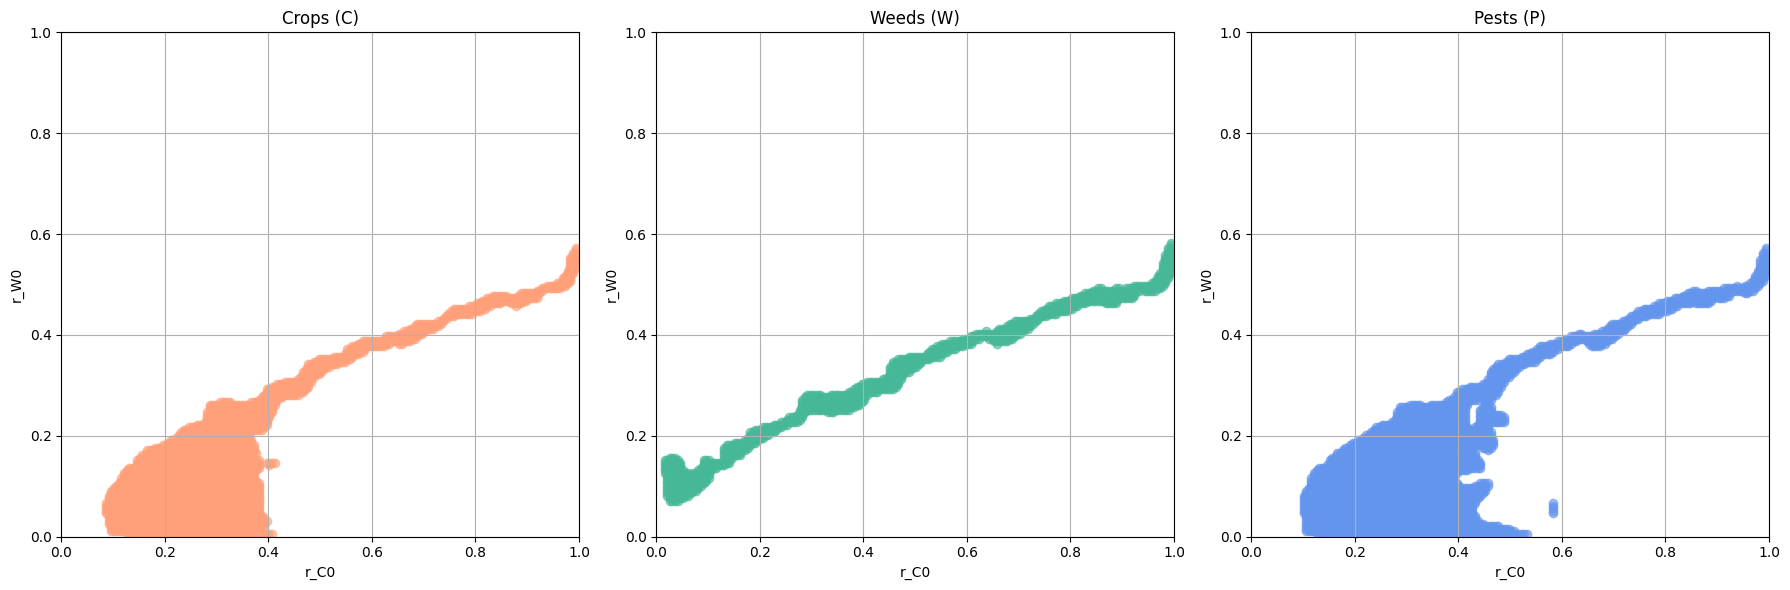
\includegraphics[width=0.8\textwidth]{model1-mk-seperate-bounds.png}
    \caption{Bounds of FarmModel-V1}
\end{figure}

Finally, we selected the set of points excluding the common points of the three species and fitted a straight line to these points. The equation of the line is \(r_{W0}=0.407r_{C0} + 0.125\). This line represents the critical point of the change in the number of species. Above and to the left of the line, the ecosystem is ultimately dominated by weeds, while the numbers of crops and pests tend to 0. Below and to the right of the line, the ecosystem ultimately forms a stable whole with a certain number of crops and pests, while the number of weeds tends to 0.

\begin{figure}[h]
    \centering
    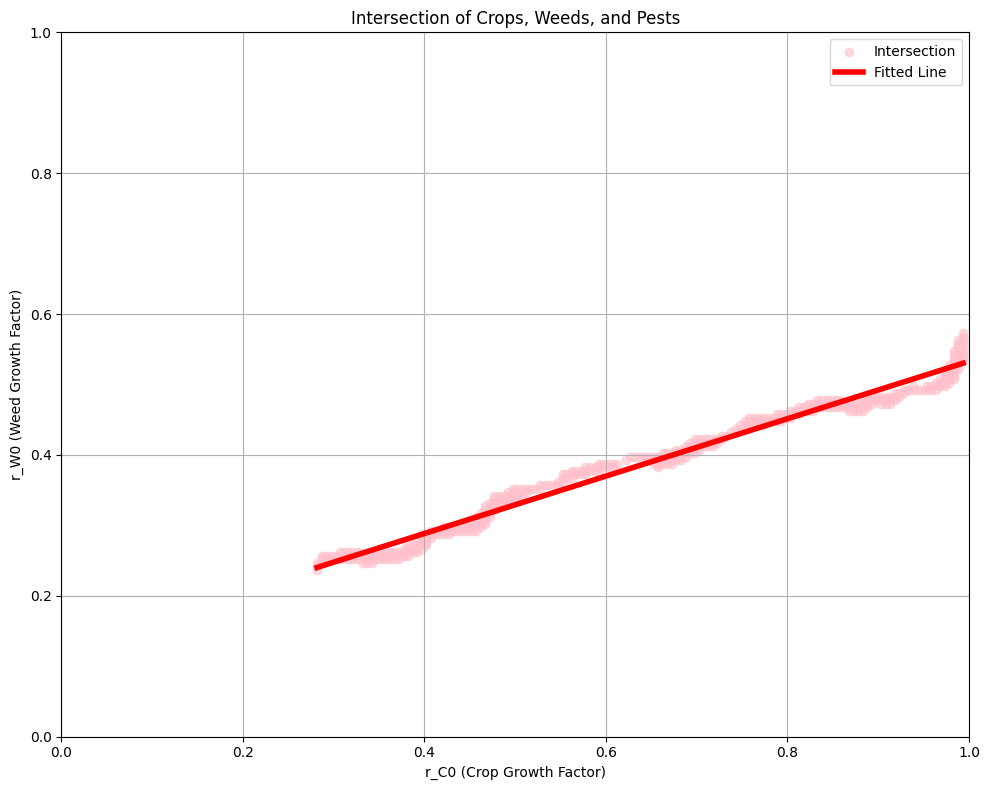
\includegraphics[width=0.4\textwidth]{model1-mk-fitted.png}
    \caption{Fitting bounds of FarmModel-V1}
\end{figure}
\textbf{About this curve, we can do some interesting analysis:}
\begin{enumerate}
    \item \textbf{Biological significance:} For ecosystems, especially some simple ones, they may be very sensitive to certain parameters. Crossing a certain threshold may cause the system to move towards an extreme. Therefore, in actual production, we need to find appropriate strategies to avoid extreme situations as much as possible.
    \item \textbf{Economic significance:} 
    \begin{enumerate}
        \item \textbf{Optimization of agricultural production:} This dividing line is helpful for optimizing agricultural production. By reasonably adjusting the growth rates of crops and weeds, the crop yield can be increased, and the competition of weeds against crops can be reduced, thereby improving the economic benefits of agriculture.

        \item \textbf{Risk management:} This dividing line is conducive to risk management. By analyzing this dividing line, we can predict the risks that agricultural production may face under different environmental conditions and thus take corresponding measures to avoid these risks.
    \end{enumerate}
\end{enumerate}

\subsubsection{FarmModel-V3}
We also conducted Monte Carlo simulations for the three stages of the FarmModel-V3 model. These three stages include: 1) removing pesticides, 2) introducing bats, and 3) introducing bees instead of bats. We paid special attention to the impact of these strategies on the quantity of crops (C), because C is a direct indicator for measuring the final economic benefits of the system and is also an indicator that farmers are most concerned about. We presented the simulation results through three - dimensional graphs respectively.

\begin{figure}[h]
    \centering
    \begin{subfigure}{.3\textwidth}
        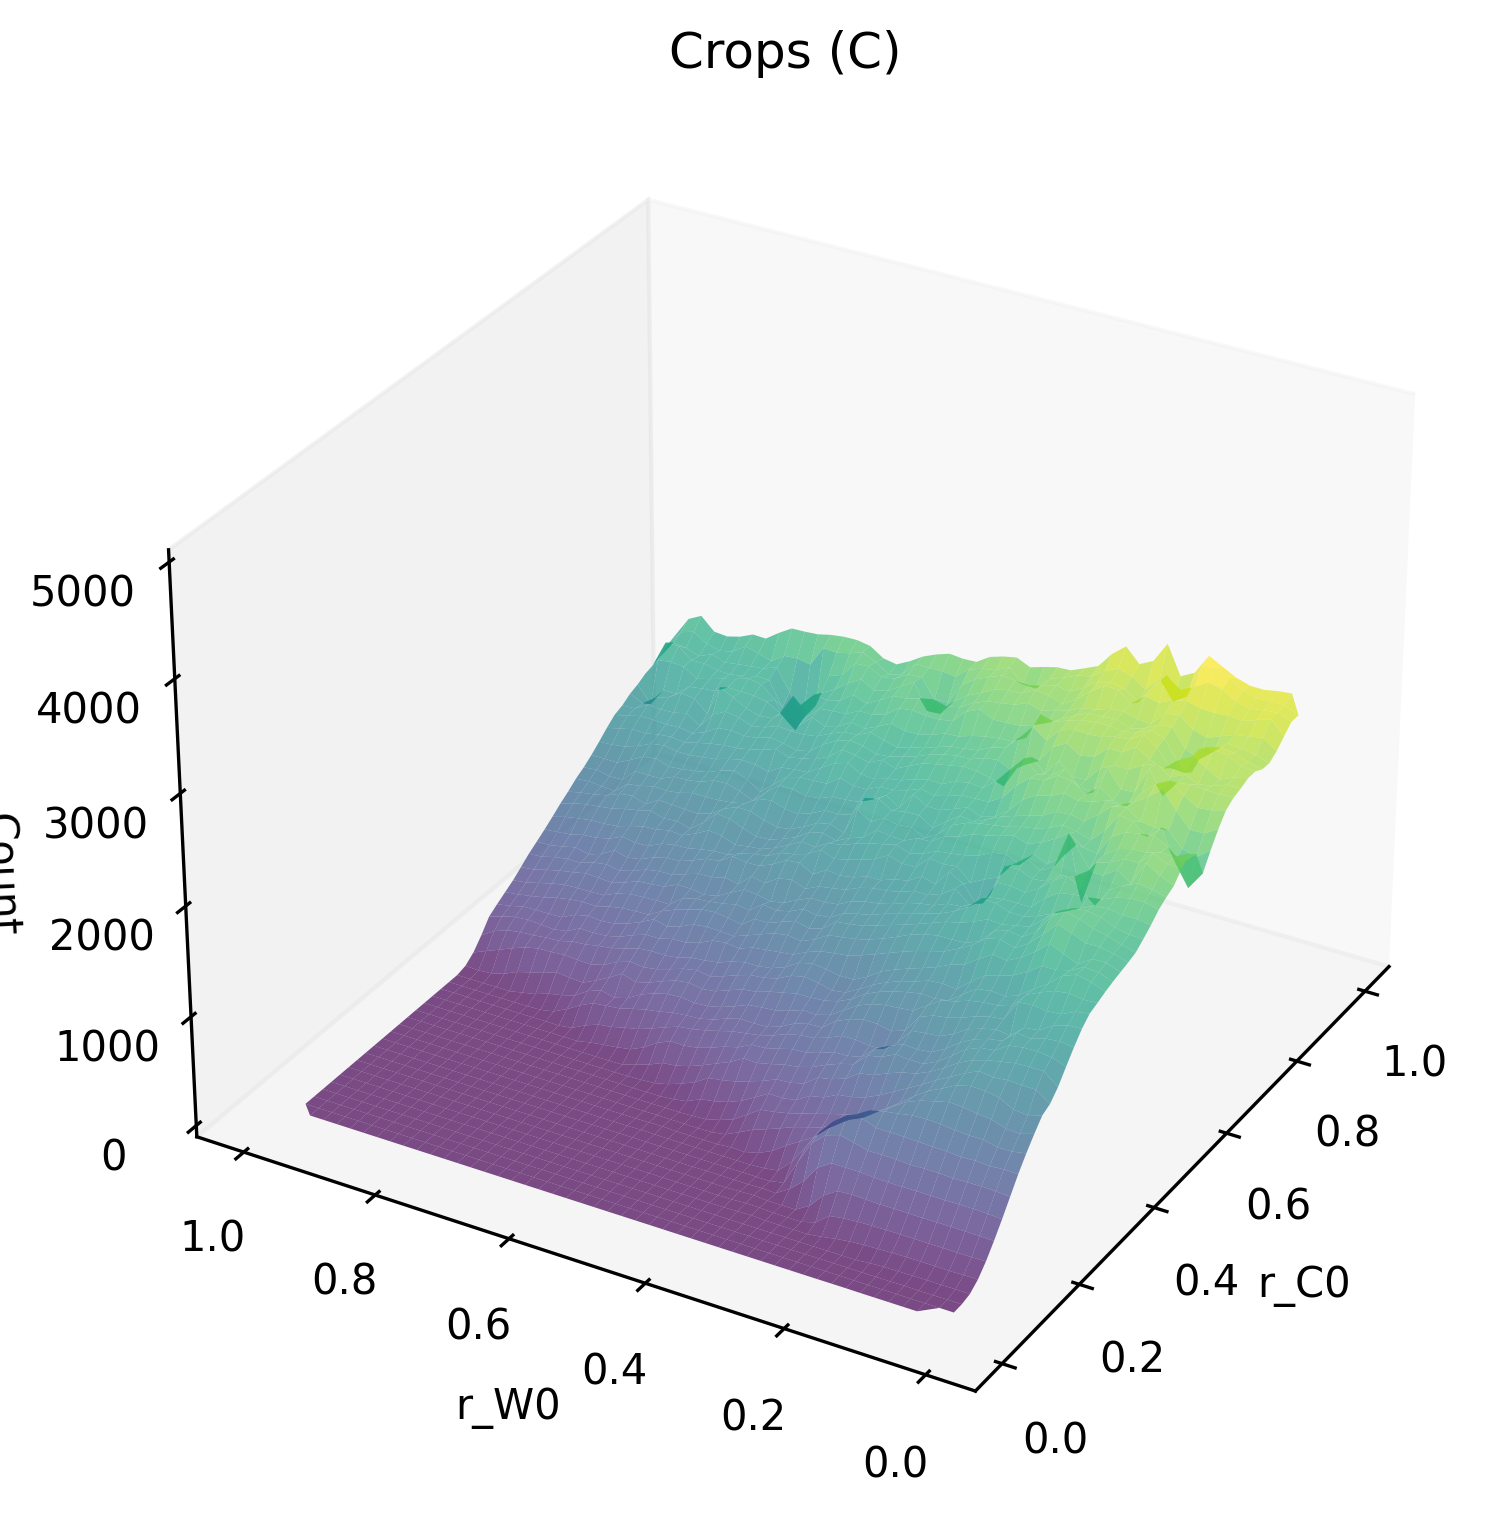
\includegraphics[width=\textwidth]{3D-Crops.png}
        \caption{Remove Pesticides}
    \end{subfigure}
    \begin{subfigure}{.3\textwidth}
        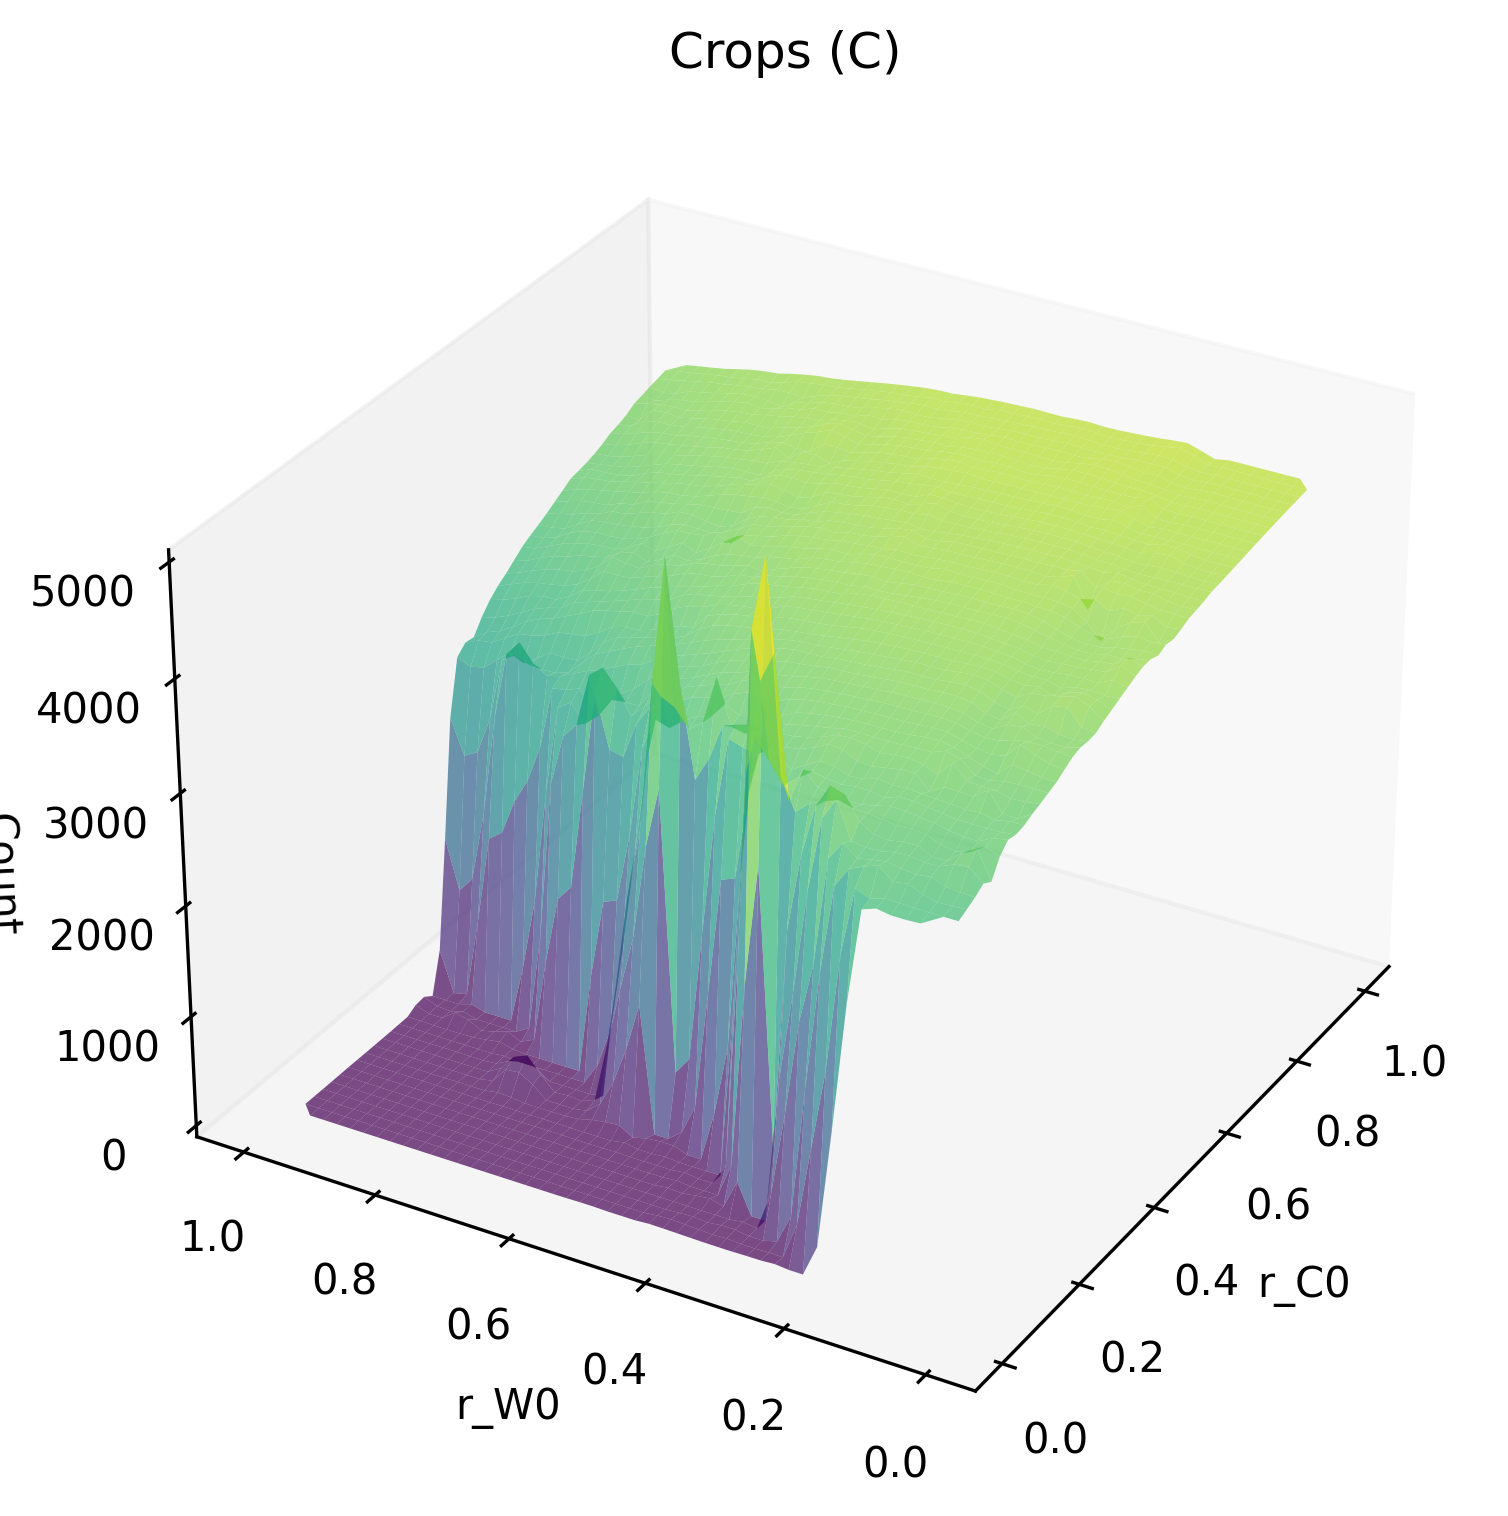
\includegraphics[width=\textwidth]{3D-Crops2.png}
        \caption{Introduce Bat}
    \end{subfigure}
    \begin{subfigure}{.3\textwidth}
        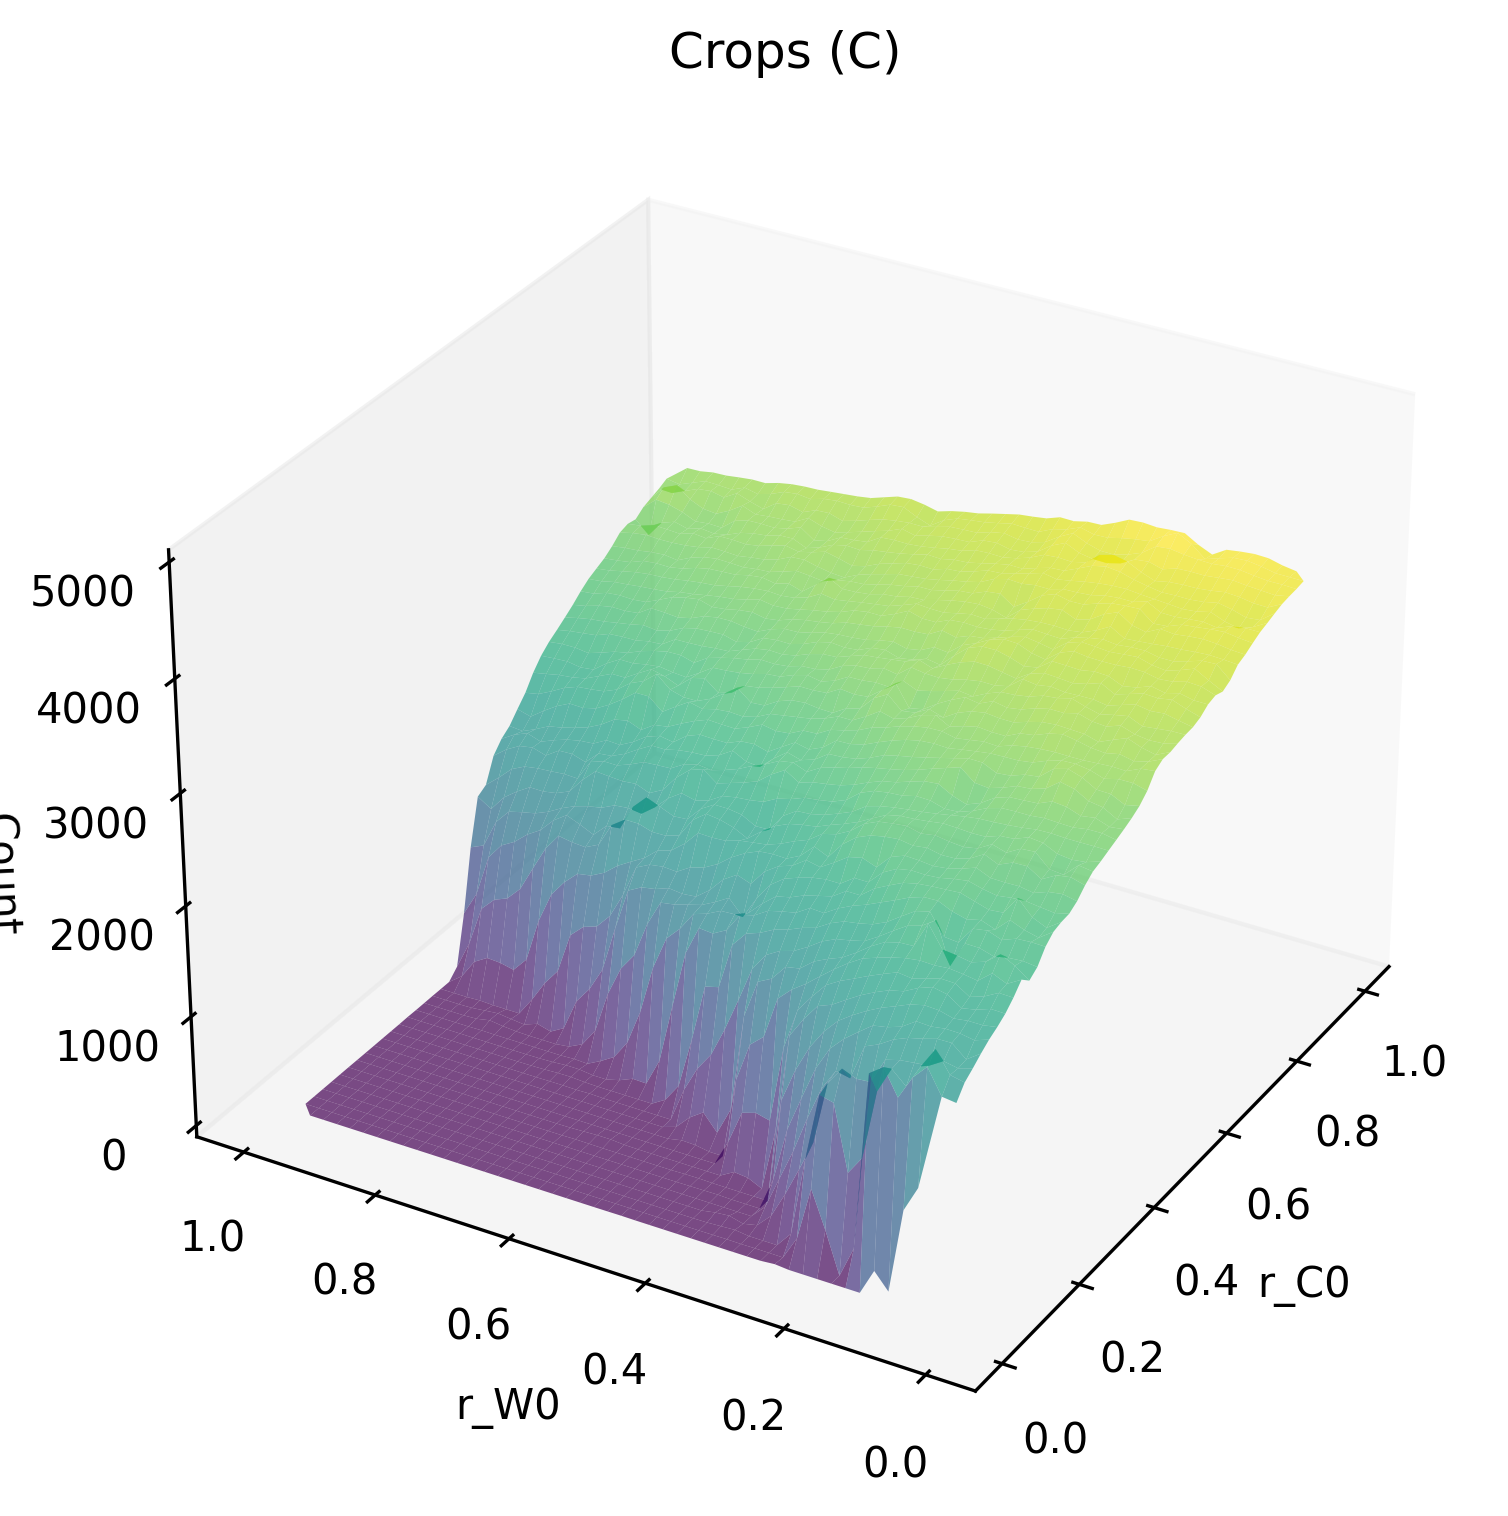
\includegraphics[width=\textwidth]{3D-Crops3.png}
        \caption{Introduce Bee}
    \end{subfigure}
\end{figure}
By observing these three - dimensional graphs, we draw the following conclusions:

\begin{enumerate}
    \item \textbf{Size of the zero - region area:} The zero - region area in Figure 1 (removing pesticides) is the largest, followed by that in Figure 3 (introducing bees), and the one in Figure 2 (introducing bats) is the smallest. This indicates that the management strategy of introducing bats is the most effective in reducing the area where the quantity of crops is below a certain threshold (e.g., 100).

    \item \textbf{Maximum height:} The maximum height in Figure 3 (introducing bees) is the highest, followed by that in Figure 2 (introducing bats), and the one in Figure 1 (removing pesticides) is the lowest. This shows that the management strategy of introducing bees is the most effective in increasing the quantity of crops.
    
\end{enumerate}

\noindent\textbf{Quantification of risk and output efficiency}

To quantify these indicators, we adopted the following methods:
\begin{enumerate}
    \item Since the results of many simulations are not exactly 0 but numbers very close to 0, for the convenience of analysis, we consider that when the final output of the system is too small (less than a certain threshold), its impact on the entire ecosystem is extremely weak and can be ignored. So we approximate it as 0.

    \item Risk indicator: 
    
    We fit a straight line to the boundary of the zero - value area, and calculate the ratio of the area above and to the left of the line (i.e., the approximate area of the zero - value area) to the total area as the risk indicator for measuring the system. The mathematical formula is as follows:
    $$
\text{Risk Index}=\frac{\text{Area where C}<100}{\text{Total Area}}
$$
Here, $C$ represents the quantity of crops, and 100 is the set threshold.
\begin{figure}[ht]
    \centering
    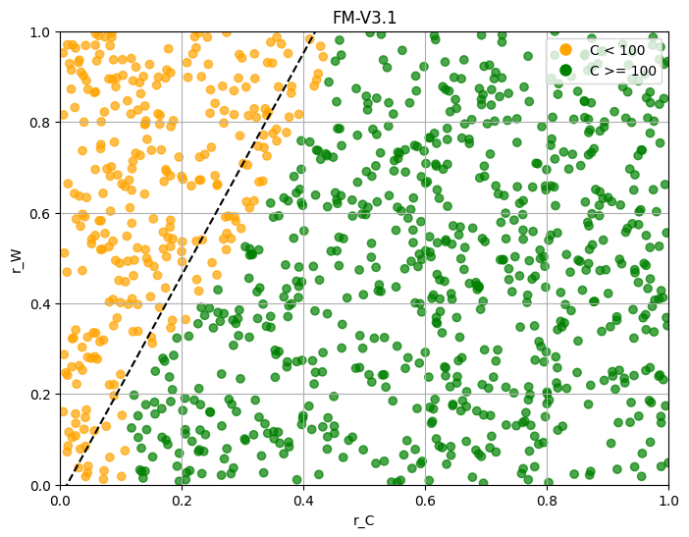
\includegraphics[width=0.3\textwidth]{image5.png}
    \caption{Risk Index of FarmModel-V3}
\end{figure}
    \item \textbf{Output efficiency indicator:} We define the output efficiency at each point as \(C/K_{C}\), where \(C\) is the quantity of crops at the corresponding point when the system reaches stability in the end, and \(K_{C}\) represents the maximum environmental capacity of crops. We sum up the output efficiencies at each point and divide by the total number for normalization to obtain the average output efficiency of the system. The mathematical formula is as follows:
    $$
    \text{Output Efficiency}=\frac{\sum C/K_{C}}{n}
    $$
    According to the above - mentioned methods, the final risks and output efficiencies of the three systems are as follows:
    \begin{enumerate}
        \item Removing pesticides: The risk index is 27.02\%, and the output efficiency is 0.26.
        \item Introducing bats: The risk index is 19.02\%, and the output efficiency is 0.79.
        \item Introducing bees: The risk index is 21.92\%, and the output efficiency is 0.54.
        
    \end{enumerate}
\end{enumerate}

Considering both the risk and the output efficiency comprehensively, we believe that the management strategy of introducing bats performs best in reducing the system risk and improving the output efficiency. The management strategy of introducing bees comes next, while the strategy of only removing pesticides performs worst in terms of these two indicators.





\subsection{Strengths and Weaknesses}
\subsubsection{Strengths}
\begin{itemize}
    \item Our model is comprehensive and integrates various scenarios
    \item After testing, the model demonstrates strong stability
    \item The model provides valuable guidance for practical production
 \end{itemize}
\subsubsection{Weaknesses}
\begin{itemize}
    \item The model does not account for the decomposition role of microorganisms
    \item The model assumptions are overly idealized and need to be further generalized to account for more common scenarios
\end{itemize}
\newpage
% 以下为信件/备忘录部分,不需要可自行去掉
% 如有需要可将整个 letter 环境移动到文章开头或中间
% 请在第二个花括号内填写标题,如「信件」(Letter)或「备忘录」(Memorandum)
\sffamily
\begin{letter}{Letter}
\BgThispage
\begin{flushleft}  % 左对齐环境,无首行缩进
\textbf{To:} Farmer tho is exploring farming practices\\
\textbf{From:} Team 2513946\\
\textbf{Date:} January 28th, 2025\\
\textbf{Subject:} Advice on the farming method and discussions on economic trade-offs and sustainability.
\end{flushleft}

As the COMAP group, we have explored the evolution of the forest-to-farm.I know that you are considering transitioning to organic farming practices, and I hope this letter can provide some insights to help you with your decision-making process. Shifting to organic agriculture is not just about economic gains but is also an essential step toward achieving long-term sustainable development.

Generally, the main approaches to organic agriculture include using organic fertilizers, adopting new planting methods, and introducing new species.From the indicator, Green Agriculture Index ,we know it is clear that different organic farming methods will have different impacts. For example, introducing new species can enhance biodiversity and improve soil fertility. Clearly, organic farming has significant positive effects on both crop yields and the ecological environment. However, implementing organic farming comes with higher costs, which can impose a certain economic burden.

To make a decision between organic farming and conventional farming, an evaluation of both the ecological and economic aspects is needed. We have provided a calculation method to assess the impacts of organic farming, which can be measured by the growth of GAI. Economically, future earnings can be simulated by data from historical planting practices. Once the results are obtained, a comparative analysis can help guide your choice.When considering sustainability and costs, different people may make different choices. To balance both, you can create an ecology-economy indicator,using the Green Agriculture Index and economic returns.This takes both sustainability and costs into account.

To incentivize farmers to protect the ecosystem through their agricultural activities,the ways are followed: first, relevant departments should offer subsidies to reduce the financial burden of implementing organic farming. Second, relevant regulations should be made, establishing environmental standards to guide farmers to reduce pesticide use. Finally, education should also be provided to increase farmers’ awareness of environmental protection.

We hope that you will consider our suggestions, enabling you to achieve high profits while contributing to the sustainability of ecosystem!

\begin{flushright}
    Yours sincerely,\\
    Team 2513946
\end{flushright}
\end{letter}

\newpage
% 参考文献,此处以 MLA 引用格式为例
\begin{thebibliography}{99}
    \bibitem{Demir2024} 
    T. Demir, "Delay Differential Equation Approach to Lotka-Volterra Predator-Prey Dynamics: Modelling Ecological Interactions with Time Delays," \textit{ResearchGate}, 2024. Available at: \url{https://www.researchgate.net/profile/Taylan-Demir-3/publication/387012361_Delay_Differential_Equation_Approach_to_Lotka-Volterra_Predator-Prey_Dynamics_Modelling_Ecological_Interactions_with_Time_Delays/links/675c13b1eea8d248be67b270/Delay-Differential-Equation-Approach-to-Lotka-Volterra-Predator-Prey-Dynamics-Modelling-Ecological-Interactions-with-Time-Delays.pdf}.
    
    \bibitem{Blake2024} 
    H. Blake, "Impact of Human Activities on Predator-Prey Dynamics in Ecological Models," \textit{ResearchGate}, 2024. Available at: \url{https://www.researchgate.net/profile/Harrison-Blake-2/publication/387730532_Impact_of_Human_Activities_on_Predator-Prey_Dynamics_in_Ecological_Models/links/6779f93000aa3770e0d735af/Impact-of-Human-Activities-on-Predator-Prey-Dynamics-in-Ecological-Models.pdf}.
    
    \bibitem{Adenekan2024} 
    T.K. Adenekan, "Systematic Study of Spatio-Temporal Dynamics in Prey-Predator Interaction Models," \textit{ResearchGate}, 2024. Available at: \url{https://www.researchgate.net/profile/Tobiloba-Adenekan/publication/386175954_Systematic_Study_of_Spatio-Temporal_Dynamics_in_Prey-Predator_Interaction_Models/links/67478025359dcb4d9d3ca157/Systematic-Study-of-Spatio-Temporal-Dynamics-in-Prey-Predator-Interaction-Models.pdf}.
    
    \bibitem{Dandekar2024} 
    R.A. Dandekar et al., "Scientific Machine Learning in Ecological Systems: A Study on the Predator-Prey Dynamics," \textit{arXiv preprint}, 2024. Available at: \url{https://arxiv.org/abs/2411.06858}.
    
\end{thebibliography}

\end{document}  % 结束
